\documentclass[11pt,a4paper]{ctexart}

\usepackage[margin=2.6cm]{geometry}
\usepackage{amsmath,amssymb,amsthm}
\usepackage{graphicx}
\usepackage{booktabs}
\usepackage{longtable}
\usepackage{array}
\usepackage{listings}
\usepackage{xcolor}
\usepackage{enumitem}
\usepackage[hidelinks]{hyperref}

\setlength{\parskip}{0.45em}
\setlength{\parindent}{0pt}
\linespread{1.28}

\newtheorem{theorem}{定理}[section]
\newtheorem{definition}[theorem]{定义}
\newtheorem{corollary}[theorem]{推论}

\lstset{
  basicstyle=\ttfamily\footnotesize,
  breaklines=true,
  breakatwhitespace=false,
  frame=single,
  rulecolor=\color{gray!45},
  backgroundcolor=\color{gray!7},
  columns=fullflexible,
  keepspaces=true,
  showstringspaces=false,
  tabsize=2,
  xleftmargin=0.4em,
  xrightmargin=0.4em,
  aboveskip=0.7em,
  belowskip=0.7em,
  extendedchars=true,
  literate=
    {ℚ}{{$\mathbb{Q}$}}1 {ℤ}{{$\mathbb{Z}$}}1 {ℕ}{{$\mathbb{N}$}}1 {ℝ}{{$\mathbb{R}$}}1
    {α}{{$\alpha$}}1 {β}{{$\beta$}}1 {γ}{{$\gamma$}}1 {δ}{{$\delta$}}1
    {ε}{{$\varepsilon$}}1 {η}{{$\eta$}}1 {θ}{{$\theta$}}1 {λ}{{$\lambda$}}1
    {μ}{{$\mu$}}1 {π}{{$\pi$}}1 {ρ}{{$\rho$}}1 {σ}{{$\sigma$}}1
    {τ}{{$\tau$}}1 {φ}{{$\varphi$}}1 {ψ}{{$\psi$}}1 {ω}{{$\omega$}}1
    {Δ}{{$\Delta$}}1 {Σ}{{$\Sigma$}}1 {Ω}{{$\Omega$}}1
    {∘}{{$\circ$}}1 {∈}{{$\in$}}1 {∉}{{$\notin$}}1 {≤}{{$\le$}}1 {≥}{{$\ge$}}1
    {≠}{{$\ne$}}1 {≈}{{$\approx$}}1 {≡}{{$\equiv$}}1 {≃}{{$\simeq$}}1
    {⊂}{{$\subset$}}1 {⊆}{{$\subseteq$}}1 {∪}{{$\cup$}}1 {∩}{{$\cap$}}1
    {→}{{$\to$}}1 {←}{{$\leftarrow$}}1 {↔}{{$\leftrightarrow$}}1 {↦}{{$\mapsto$}}1
    {⟺}{{$\Longleftrightarrow$}}1 {⟹}{{$\Longrightarrow$}}1
    {⟸}{{$\Longleftarrow$}}1 {⟶}{{$\longrightarrow$}}1 {↓}{{$\downarrow$}}1
    {∀}{{$\forall$}}1 {∃}{{$\exists$}}1 {¬}{{$\neg$}}1 {∧}{{$\wedge$}}1 {∨}{{$\vee$}}1
    {∑}{{$\sum$}}1 {∏}{{$\prod$}}1 {∞}{{$\infty$}}1 {√}{{$\sqrt{\ }$}}1
    {⌊}{{$\lfloor$}}1 {⌋}{{$\rfloor$}}1 {⟨}{{$\langle$}}1 {⟩}{{$\rangle$}}1
    {‖}{{$\|$}}1 {…}{{$\ldots$}}1
    {₀}{{$_0$}}1 {₁}{{$_1$}}1 {₂}{{$_2$}}1 {₃}{{$_3$}}1 {₄}{{$_4$}}1
    {ᵢ}{{$_i$}}1 {ⱼ}{{$_j$}}1 {ⁿ}{{$^n$}}1 {²}{{$^2$}}1 {³}{{$^3$}}1 {¹}{{$^1$}}1
    {×}{{$\times$}}1 {·}{{$\cdot$}}1 {∎}{{$\blacksquare$}}1,
}

\title{可解释性 = 可编码性\\[0.3em]\large 神经网络可解释性的层论基础}
\author{Wenxu Shu}
\date{}

\begin{document}
\maketitle
\bigskip

\section*{摘要}

神经网络的"黑箱"问题长期停留在一个形容词上：我们说不出它为什么给这个答案。本文把它换成一个命题。

我们把网络建模成\textbf{逐层映射族}，层塔是有限、一维、严格递减的阈值链。可解释性被定义为：整条层族能否由一个\textbf{单层源对象}沿塔消解生成。在这个模型下我们证明：

\textbf{可解释 \ensuremath{\Longleftrightarrow} 可编码。} 相干网络态与单层对象之间存在一对互逆映射，编码是单射。于是"黑箱"有了一个肯定式定义：\textbf{不存在能生成它的源}——不是我们看不懂它，是它没有代码。

第二，这个判据的\textbf{代价是可算的}。对 ReLU 族，坍缩跨度有精确闭式 \texttt{gap = (c/a + 1)²}，标准 ReLU 的 gap 恰为 1（不是 0）；多层复合服从一条非加非乘的律 \texttt{\ensuremath{\sqrt{\mathrm{gap}}}(g\ensuremath{\circ}f) = \ensuremath{\sqrt{\mathrm{gap}}}(f) + (\ensuremath{\sqrt{\mathrm{gap}}}(g)\ensuremath{-}1)/\ensuremath{a_{1}}}。由此得到容量的精确边界：在盒 \texttt{[\ensuremath{-}B,B]} 上，可分辨点数 \texttt{max N = \ensuremath{\lfloor}2B/\ensuremath{\sqrt{\mathrm{g}}}\ensuremath{\rfloor} + 1}，且等距网格达到它。

第三，一个反直觉的推论：\textbf{可解释性与泛化不是同向的}。gap 同时是容量的倒数，所以 gap 越大泛化越容易、越不可解释。\textbf{黑箱不是缺陷，是泛化的来源}——它不能修复（信息已丢），也不该修复（修好了就没有泛化）。

第四，我们对近期用层论做可解释性的外部方案给出划界：同一个 \texttt{\ensuremath{b_{1}}} 公式，建在\textbf{观察层塔}上恒为零（方格全部交换），建在\textbf{计算网格}上才计数扩张层。\textbf{\texttt{\ensuremath{b_{1}}} 是 site 的函数，不是网络的属性。}

全部结论在 Lean 4 + Mathlib 中机械检验：零 \texttt{sorry}，不使用经典逻辑，全程有理数。这不是工程附注，是内容的一部分（§1.5）。

\textbf{关键词：} 可解释性；层论；编码；ReLU；坍缩跨度；构造性数学；Lean 4

\bigskip

\section*{Abstract}

The "black box" problem in neural networks has long remained an adjective: we cannot say why a network gives the answer it gives. This paper turns it into a proposition.

We model a network as a \textbf{layer-wise family of maps}, with the layer ladder being a finite, one-dimensional, strictly decreasing chain of thresholds. Interpretability is defined as: whether the entire layer family can be generated by a \textbf{single-layer source} via resolution along the ladder. Under this model we prove:

\textbf{Interpretable \ensuremath{\Longleftrightarrow} encodable.} Coherent network states and single-layer objects are related by a pair of mutually inverse maps, and the encoding is injective. "Black box" thereby acquires a positive definition: \textbf{there exists no source that generates it} — not that we fail to understand it, but that it has no code.

Second, the \textbf{cost of this criterion is computable}. For the ReLU family the collapse span has a closed form \texttt{gap = (c/a + 1)²}; for the standard ReLU the gap is exactly 1 (not 0). Composition follows a law that is neither additive nor multiplicative: \texttt{\ensuremath{\sqrt{\mathrm{gap}}}(g\ensuremath{\circ}f) = \ensuremath{\sqrt{\mathrm{gap}}}(f) + (\ensuremath{\sqrt{\mathrm{gap}}}(g)\ensuremath{-}1)/\ensuremath{a_{1}}}. This yields an exact capacity bound: in the box \texttt{[\ensuremath{-}B,B]} the number of distinguishable points satisfies \texttt{max N = \ensuremath{\lfloor}2B/\ensuremath{\sqrt{\mathrm{g}}}\ensuremath{\rfloor} + 1}, attained by the uniform grid.

Third, a counterintuitive corollary: \textbf{interpretability and generalization do not point the same way}. The gap is also the reciprocal of capacity, so a larger gap means easier generalization and poorer interpretability. \textbf{The black box is not a defect but the source of generalization} — it cannot be repaired (the information is already lost), and should not be (repairing it destroys generalization).

Fourth, we delineate the scope of recent work that applies sheaf theory to interpretability: the same \texttt{\ensuremath{b_{1}}} formula is identically zero on the \textbf{observation ladder} (every square commutes), and only counts expanding layers on the \textbf{computation grid}. \textbf{\texttt{\ensuremath{b_{1}}} is a function of the site, not a property of the network.}

All results are machine-checked in Lean 4 + Mathlib: zero \texttt{sorry}, no classical logic, entirely over the rationals. This is not an engineering footnote but part of the content (§1.5).

\textbf{Keywords:} interpretability; sheaf theory; encoding; ReLU; collapse span; constructive mathematics; Lean 4

\bigskip

\section{引言}

\subsection{一个形容词，还是一个对象？}

"这个神经网络可解释吗？"

这个问题今天通常得到三种回答：一张显著图、一组概念向量、或者一个分数。三种都不是回答——它们说的是"这里有点东西"，不是"这是可解释的"。

\textbf{可解释性被当作一种程度}：有些层更容易理解，有些更难。

本文主张它不是程度，是\textbf{结构}。而且精确地等于一件事：

\begin{quote}
\textbf{存在一个有限的编码。}
\end{quote}

用一句话说就是：\textbf{能被写下来的东西，才谈得上被理解。}

\subsection{三条主张}

本文给出三条形式化的结论，全部在 Lean 4 中机械检验（零 \texttt{sorry}，不使用经典逻辑，全程 \ensuremath{\mathbb{Q}}）。

\textbf{三条主张不是并列的，是一条链：}

\begin{lstlisting}
主张一（判据）—— 可解释性有肯定式定义：可解释 ⟺ 可编码
        ↓  这个判据不是空话：每一层都要付代价
主张二（代价）—— 代价是一个可算的数：gap = (c/a+1)²
        ↓  有了判据和代价，才能对外部方法的位置说清楚
主张三（划界）—— 诊断该建在哪里：观察层塔 vs 计算网格
\end{lstlisting}

一条判据、一个可算的代价、一个对外部方法的划界——缺任何一条，前一条都只是修辞。

\textbf{主张一：可解释性有一个肯定式的判据（§4–§5）。}

我们把网络建模成\textbf{逐层映射族}（§4.2），层塔是一个有限、一维、严格递减的序列。在这个模型下：

\begin{lstlisting}
网络态相干  ⟺  存在一个源对象，整条层族是它沿塔的消解像
\end{lstlisting}

而"编码"与"解码"是一对互逆映射，因此这个源是\textbf{唯一且确定的}：

\begin{lstlisting}
encode : 单层对象 ⟶ 层族       decode : 层族 ⟶ 单层对象
decode ∘ encode = id            encode ∘ decode = id  （相干时）
encode 是单射
\end{lstlisting}

于是：

\begin{quote}
\textbf{可解释 \ensuremath{\Longleftrightarrow} 可编码。}
\end{quote}

黑箱因此有了一个肯定式的定义：\textbf{没有代码。} 不是"我们看不懂它"，是"不存在能生成它的源"。

\textbf{主张二：这个判据的"代价"是一个可算的数（§6）。}

对最简单的具体网络族

\begin{lstlisting}
f(x) = max 0 (a·x − c),   x ∈ [−1, 1]
\end{lstlisting}

的坍缩跨度（gap）有精确闭式：

\begin{lstlisting}
gap = (c/a + 1)²
\end{lstlisting}

两端：

\begin{center}\small
\begin{tabular}{lll}
\toprule
c/a & gap & 含义 \\
\midrule
0 & \textbf{1} & 标准 ReLU \\
1 & \textbf{4} & 杀死整个输入盒 \\
\bottomrule
\end{tabular}
\end{center}

\textbf{标准 ReLU 的 gap 是 1，不是 0。} 任何 ReLU 层都至少损失 1 个单位的距离——负半轴整段被压成 0。

而多层复合有一个\textbf{非加非乘}的律（§6.6）：

\begin{lstlisting}
√gap(g∘f) = √gap(f) + (√gap(g) − 1) / a₁
\end{lstlisting}

单位权重时最干净：\texttt{\ensuremath{\sqrt{\mathrm{gap}}}(g\ensuremath{\circ}f) = \ensuremath{\sqrt{\mathrm{gap}}}(f) + \ensuremath{\sqrt{\mathrm{gap}}}(g) \ensuremath{-} 1}。那个 \texttt{\ensuremath{-}1} 就是标准 ReLU 那个 \texttt{1} 的减法形式。

这个数还有第二面（§7）：\textbf{gap 同时是分辨率的闸门。} 在盒 \texttt{[\ensuremath{-}B,B]} 上 gap 为 \texttt{g}，能分辨的网格点数 \texttt{N < B/\ensuremath{\sqrt{\mathrm{g}}}}。于是：

\begin{quote}
\textbf{gap 大 = 简单、泛化容易，同时 = 信息丢得多、不可解释。可解释性与泛化不是同向的。}
\end{quote}

深度 ReLU 能泛化，部分原因正是它丢信息——\texttt{gap} 就是它丢了多少。

\textbf{主张三：sheaf 诊断该建在哪里，是可以论证的（§8）。}

近期工作把层论直接用于可解释性：在改述图上建 cellular sheaf，用 Laplacian 拆分内容子空间与 \texttt{\ensuremath{H^{1}}} 方向（Grant \& Wang, NeurIPS 2026）。他们报告 \texttt{\ensuremath{b_{1}} = N(L\ensuremath{-}1)} 个 1-循环，其 harmonic mass 与 steering fragility 强相关。

我们问一个更窄的问题：\textbf{在我们这套形式化里，那个 \texttt{\ensuremath{b_{1}}} 是什么？}

答案是两条：

\begin{enumerate}
\item \textbf{观察层塔的第一贝蒂数恒为 0}（定理 8.1；根源是定理 4.8）：不是网络的属性，是观测方式的属性。所以\textbf{诊断不能建在那里}。
\item \textbf{在计算网格上，方格交换 \ensuremath{\Longleftrightarrow} 层变换不放大 \ensuremath{\delta}-等价}（定义 8.2、定理 8.4），于是 \texttt{\ensuremath{b_{1}}} 计数\textbf{扩张层}。
\end{enumerate}

\textbf{本文不复现他们的实验，也不与他们竞争。} 本文做的是划界、翻译与计算。

\textbf{合起来看：} 主张一把"黑箱"从一个形容词变成一个否定式的命题（不存在代码）；主张二把"压缩得厉害"从一个比喻变成一个数；主张三把"sheaf 诊断该建在哪里"从一个品味问题变成一个可以证明的问题（同一个 \texttt{\ensuremath{b_{1}}}，建在不同 site 上，一个是恒零，一个计数扩张层）。三条都是形式化过的，不是猜想。

\textbf{所以本文的贡献不是"又一个可解释性指标"。} 而是：

\begin{quote}
\textbf{可解释性有一个结构判据（可编码），这个判据的代价可算（gap），而且已有的 sheaf 诊断不能建在观察层塔上（\texttt{\ensuremath{b_{1}} \ensuremath{\equiv} 0}）。三者合起来，给出"可解释性 = 可编码性"的层论基础。}
\end{quote}

判据回答"是不是"，代价回答"值多少"，划界回答"该在哪里测"。\textbf{只有第一条，本文是一篇定义文章；只有前两条，是一篇度量文章；三条都有，才是一个基础。}

\subsection{这三条背后是一个公理}

上述框架不是一组自选定义，而是\textbf{一个公理系统的模型}。公理只有一条主干：

\begin{quote}
\textbf{A0（自指）}：存在映射 \texttt{\ensuremath{\alpha} \ensuremath{\to} (\ensuremath{\alpha} \ensuremath{\to} Bool)}。
\end{quote}

\textbf{先澄清一个用词。} A0 在技术上其实是\textbf{定义}而不是公理：每个类型 \texttt{\ensuremath{\alpha}} 都自动带一个 \texttt{SelfRef \ensuremath{\alpha}} 实例（取常函数即可，见附录 A.1），所以不需要"假设"它存在。我们仍然叫它"公理"，理由是\textbf{它规定了后面一切的读法}——从这条映射出发，洞是必然而不是偶然；换成别的出发点（例如只有外部观测），洞就不出现。这个称呼的选择在附录 A.1 有完整说明。

A0 无条件地产生一个洞——任何 \texttt{observe} 都漏掉至少一个判定（定理 2.1）。这是康托尔对角线，也是 Lawvere 不动点定理的特例，但解读不同：

\begin{center}\small
\begin{tabular}{lll}
\toprule
 & 自指导致 & 态度 \\
\midrule
罗素 & 矛盾 & 禁止 \\
哥德尔 & 不完备 & 接受 \\
Lawvere & 不动点 & 存在 \\
\textbf{本文} & \textbf{洞} & \textbf{它就是"我"} \\
\bottomrule
\end{tabular}
\end{center}

\textbf{加上有限（A1）}，洞变成可计数的（推论 2.2）。层塔是它的一个具体实例（§2.1、附录 A）：\texttt{L.m} 层只能给出 \texttt{L.m} 个分辨者，分辨空间却有 \texttt{2\textasciicircum{}\{L.m\}} 种——\textbf{必漏}。附录 A 给出完整推导。

\textbf{但 A0/A1 不参与 §4–§8 的任何证明。} 这一点由 Lean 的编译顺序直接保证：\texttt{SelfRef} 与 \texttt{entropy} 定义在 \texttt{Ego.lean} 第 12960 行之后，而论文的定理（\texttt{Coherent}、\texttt{encode}、\texttt{IsGap}、\texttt{b1} 系列）全部在它之前，Lean 不允许前向引用。所以\textbf{删掉附录 A，论文的定理一条都不会少。}

它们回答的是另一个问题：\textbf{为什么这个模型值得选}——为什么层塔是有限、一维、严格递减的链，而不是别的结构。这是动机，不是前提。

\subsection{与已有工作的关系}

\textbf{拓扑数据分析。} 用持久同调分析神经网络是成熟方向（Naitzat et al., JMLR 2020；Neural Persistence, ICLR 2019）。本文与之一致：§2.5 的三界读数在结构上是谱的层析。区别在于本文不做经验测量，而是证明读数的结构性质。

\textbf{Sheaf 方法。} Grant \& Wang (2026) 把 sheaf 用于改述一致性；也有工作用 gauge 理论刻画叠加（2026）。本文与它们的区别在 §8：\textbf{我们的 site 是一条链，所以粘合公理退化为定理}（§3），代价是 \texttt{\ensuremath{H^{1}} \ensuremath{\equiv} 0}。

\textbf{压缩与可解释性。} "可解释 \ensuremath{\approx} 压缩"的直觉已有先例（MDL 原则；MDL-SAE, 2024）。本文的区别在于\textbf{定理形式}：不是"越小越好"的排行榜，而是"存在编码 \ensuremath{\Longleftrightarrow} 相干"的等价命题。

\textbf{形式化。} 本文的全部结论在 Lean 4 中机械检验。据我们所知，AI 可解释性领域尚无同等规格的构造性形式化。

\subsection{为什么是 \ensuremath{\mathbb{Q}}，为什么是构造性}

本文全程使用有理数，不使用实数，不使用经典逻辑。

这不是技术偏好，是\textbf{内容的一部分}：

\begin{itemize}
\item \textbf{符号必须能写完。} \ensuremath{\mathbb{Q}} 的每个元素是一对有限整数；\ensuremath{\mathbb{R}} 的绝大多数元素不是。§2.5 把这句话变成定理（连分数编码）。
\item \textbf{洞必须是可数的。} §2.1 的 \texttt{entropy f = 2\textasciicircum{}\{|\ensuremath{\alpha}|\} \ensuremath{-} |image f|} 只有在有限处才有意义。
\item \textbf{拒绝连续统是拒绝无穷可分。} 每一次除法都留残差，所以不存在无限下降的正整数链（\texttt{no\_infinite\_descent}）。
\end{itemize}

\textbf{"有限"在这里不是约束，是资格。}

\subsection{论文结构}

\begin{center}\small
\begin{tabular}{ll}
\toprule
节 & 内容 \\
\midrule
§2 & 状态、读数、层塔的形式化基础；自指公理 \\
§3 & 紧层论：为什么 site 是一条链，代价是什么 \\
§4 & 两个判据：结构判据（\texttt{Coherent}）与定量判据（\texttt{CoherentMap}） \\
§5 & \textbf{主定理：可解释 = 可编码} \\
§6 & gap 的精确值：单层闭式、复合律、四条推论 \\
§7 & gap 的延伸：计数界、精确容量、斜率不变量、\ensuremath{\eta}-近似、多维 \\
§8 & 诊断该建在哪里：观察层塔 vs 计算网格（与外部方案的对话） \\
§9 & 相关工作、局限、四条可证伪的预言 \\
附录 A & 自指公理 A0 + A1 \ensuremath{\Longrightarrow} 洞 \\
附录 B & Lean 定理索引 \\
\bottomrule
\end{tabular}
\end{center}

\bigskip

\section{基础：状态、读数与层塔}

\subsection{一切的起点：自指}

本文的框架建立在一个单一的原始事实上：\textbf{系统能对自己作判定。}

把它写成公理：

\textbf{公理 A0（自指）.} 存在一个映射 \texttt{observe : \ensuremath{\alpha} \ensuremath{\to} (\ensuremath{\alpha} \ensuremath{\to} Bool)}。

\begin{lstlisting}
structure SelfRef (α : Type*) where
  observe : α → resolveSpace α
\end{lstlisting}

（其中 \texttt{resolveSpace \ensuremath{\alpha}} 就是 \texttt{\ensuremath{\alpha} \ensuremath{\to} Bool}——"用 \ensuremath{\alpha} 的每个元素作一次是/否判定"。）

\textbf{这不是要回避的东西，是起点。} 而它的后果是众所周知的：

\textbf{定理 2.1（洞）.} 对\textbf{任意}类型的\textbf{任意} \texttt{observe}，

\begin{lstlisting}
∃ d : α → Bool,  ∀ a : α,  d ≠ observe a
\end{lstlisting}

\begin{lstlisting}
theorem diagonal_hole {α : Type*} (f : α → resolveSpace α) :
    ∃ d : resolveSpace α, ∀ a : α, d ≠ f a
\end{lstlisting}

\textbackslash\{\}emph\{证明.\} 取 \texttt{d := fun a => \ensuremath{\neg}(f a a)}（康托尔对角线）。

\textbf{这条定理没有任何假设}——不需要有限性，不需要可判定性。它是纯逻辑的。

\textbf{推论 2.2（有限时洞可量化）.} 若 \texttt{\ensuremath{\alpha}} 有限，则漏得至少一个：

\begin{lstlisting}
theorem entropy_positive [Fintype α] [DecidableEq α] [Nonempty α]
    (f : α → resolveSpace α) : 0 < entropy f
\end{lstlisting}

其中 \texttt{entropy f := 2\textasciicircum{}\{|\ensuremath{\alpha}|\} \ensuremath{-} |image f|}。

\textbf{要在本文里记住这两条的分工}：A0 无条件给洞；A1（有限）把洞变成可计数的。

\subsection{状态}

\textbf{定义 2.3（状态）.} \texttt{n} 维状态是一个量向量加一个相位：

\begin{lstlisting}
structure StateQuant (n : ℕ) where
  val : Fin n → ℚ
  phase : Phase

inductive Phase where
  | positive | negative | neutral
\end{lstlisting}

\textbf{为什么是 \ensuremath{\mathbb{Q}} 而不是 \ensuremath{\mathbb{R}}？}

因为\textbf{符号必须能写完}。\ensuremath{\mathbb{Q}} 的每个元素是一对有限整数；\ensuremath{\mathbb{R}} 的绝大多数元素不是。§2.5 会把这句话变成一个定理（连分数编码）。

\textbf{为什么是两个坐标？}

这不是选择，是被群作用逼出来的——下一小节说明。

\subsection{为什么恰好是这两个坐标}

考虑两个自然的对称群：

\begin{itemize}
\item \textbf{缩放群} \texttt{\ensuremath{\mathbb{Q}}\textasciicircum{}\ensuremath{\times}}：把状态整体推远或拉近；
\item \textbf{翻转群} \texttt{\ensuremath{\mathbb{Z}}/2}：正负互换，中性不动。
\end{itemize}

\textbf{定理 2.4（坐标唯一性，六条）.}

\begin{lstlisting}
theorem coordinates_unique
\end{lstlisting}

\begin{center}\small
\begin{tabular}{lll}
\toprule
条 & 内容 & 定理 \\
\midrule
（1）完备 & 两投影联合单射 & \texttt{val\_phase\_complete} \\
（2）必需 & 单独任一投影不够 & \texttt{val\_not\_sufficient}、\texttt{phase\_not\_sufficient} \\
（3）对角 & \texttt{\ensuremath{\mathbb{Q}}\textasciicircum{}\ensuremath{\times}} 只在 \texttt{val} 非平凡；\texttt{\ensuremath{\mathbb{Z}}/2} 只在 \texttt{phase} 非平凡 & \texttt{scale\_phase\_trivial}、\texttt{flip\_val\_trivial}（两条 \texttt{rfl}）+ 两个见证 \\
（4）忠实 & 两个群在各自坐标上不偷懒 & \texttt{scale\_faithful}、\texttt{flip\_faithful} \\
（5）不可再分 & \texttt{\ensuremath{\mathbb{Z}}/2}-不变的函数分不开正负 & \texttt{no\_sign\_refinement} \\
（6）齐次 & 一维非零同相位态全同轨道 & \texttt{one\_dim\_one\_orbit} \\
\bottomrule
\end{tabular}
\end{center}

\textbf{第（3）条是整个可分性的内容}，而它的两个方向各是一条 \texttt{rfl}：

\begin{lstlisting}
theorem scale_phase_trivial (c : ℚ) (x : StateQuant n) : (scale c x).phase = x.phase := rfl
theorem flip_val_trivial (x : StateQuant n) : (flipState x).val = x.val := rfl
\end{lstlisting}

\textbf{平凡性由定义直接成立}——这正是"坐标是按群作用设计的"的证据。

\textbf{第（5）条最有意思}：任何 \texttt{\ensuremath{\mathbb{Z}}/2}-不变的函数都无法区分正与负。

\begin{lstlisting}
theorem no_sign_refinement {β : Type*} (f : Phase → β)
    (hf : ∀ p, f (flipPhase p) = f p) : f .positive = f .negative
\end{lstlisting}

这意味着 \texttt{\{+, \ensuremath{-}\}} 是\textbf{单个轨道}，再往下切就没有群论根据了。\textbf{"二值"之所以是二值，是因为 \texttt{\ensuremath{\mathbb{Z}}/2} 只给了两个轨道。}

\subsection{距离}

\textbf{定义 2.5（距离）.} 两个状态的公共维数上的平方差之和：

\begin{lstlisting}
def commonDist {m n : ℕ} (x : StateQuant m) (y : StateQuant n) : ℚ :=
  ∑ i : Fin (min m n), (x.val (embedLeft i) − y.val (embedRight i))²
\end{lstlisting}

\textbf{一维时它就是平方差}：

\begin{lstlisting}
theorem commonDist_one (x y : StateQuant 1) :
    commonDist x y = (x.val 0 - y.val 0) ^ 2
\end{lstlisting}

（§6 起，凡涉及一维的讨论，都直接用 \texttt{(x \ensuremath{-} y)²} 这个等价写法。）

\textbf{它满足一条关键的齐次性：}

\textbf{定理 2.6（保角性）.}

\begin{lstlisting}
commonDist (c·x) (c·y) = c² · commonDist x y
\end{lstlisting}

\begin{lstlisting}
theorem scale_commonDist (c : ℚ) (x y : StateQuant n) :
    commonDist (scale c x) (scale c y) = c ^ 2 * commonDist x y
\end{lstlisting}

\textbf{这里有一个容易犯的错}（本文初稿就犯过）：以为保角性 \texttt{D(c\ensuremath{\cdot}v) = \ensuremath{c^{2}}\ensuremath{\cdot}D(v)} 能确定平方和。

\textbf{不能。} 任何二次型都是 2 次齐次的，所以保角性对\textbf{所有}二次型成立——它筛不掉任何东西。

真正的刻画需要另外两条\textbf{公理}：

\begin{center}\small
\begin{tabular}{lll}
\toprule
公理 & 内容 & 直觉 \\
\midrule
\textbf{(i) 支撑不交可加} & 若 \texttt{v}、\texttt{w} 在每个坐标上至多一个非零，则 \texttt{D(v + w) = D(v) + D(w)} & 各部分独立贡献 \\
\textbf{(ii) 坐标置换不变} & 换掉坐标顺序不改变 \texttt{D} & 没有偏爱某个维度 \\
\bottomrule
\end{tabular}
\end{center}

\textbf{定理 2.7（平方和的唯一性，n 维）.} 设 \texttt{D} 是 \texttt{n} 维二次型

\begin{lstlisting}
D(v) = Σᵢⱼ Mᵢⱼ vᵢ vⱼ
\end{lstlisting}

若满足 (i) 与 (ii)，则

\begin{lstlisting}
D(v) = α · Σᵢ vᵢ²
\end{lstlisting}

\begin{lstlisting}
theorem quadForm_is_squared_norm {n : ℕ} (M : Fin n → Fin n → ℚ) (hn : 0 < n)
    (hadd : ∀ (v w : Fin n → ℚ), (∀ i, v i = 0 ∨ w i = 0) →
      quadForm M (v + w) = quadForm M v + quadForm M w)
    (hswap : ∀ (i j : Fin n) (v : Fin n → ℚ),
      quadForm M (fun k => v (swapCoord i j k)) = quadForm M v) :
    ∃ α : ℚ, ∀ v : Fin n → ℚ, quadForm M v = α * ∑ i, v i ^ 2
\end{lstlisting}

\textbackslash\{\}emph\{证明.\} 分三步，\textbf{维度在这里不起作用}。

\textbf{第一步（可加 \ensuremath{\Longrightarrow} 交叉项相消）.} 取 \texttt{v = \ensuremath{e_{i}}\ensuremath{\cdot}1}、\texttt{w = \ensuremath{e_{j}}\ensuremath{\cdot}1}（\texttt{i \ensuremath{\ne} j}，支撑不交）：

\begin{lstlisting}
D(eᵢ + eⱼ) = Mᵢᵢ + Mᵢⱼ + Mⱼᵢ + Mⱼⱼ
D(eᵢ) + D(eⱼ) = Mᵢᵢ + Mⱼⱼ
\end{lstlisting}

相减得 \texttt{\ensuremath{M_{ij}} + \ensuremath{M_{ji}} = 0}（\texttt{quadForm\_offdiag}）。

\textbf{第二步（置换不变 \ensuremath{\Longrightarrow} 对角元相等）.} 交换坐标 \texttt{i, j} 把 \texttt{\ensuremath{e_{i}}} 送成 \texttt{\ensuremath{e_{j}}}（\texttt{basisVec\_comp\_swap}），于是 \texttt{D(\ensuremath{e_{j}}) = D(\ensuremath{e_{i}})}，即 \texttt{\ensuremath{M_{jj}} = \ensuremath{M_{ii}}}。

\textbf{第三步（反对称部分归零）.} 设 \texttt{\ensuremath{\alpha} = \ensuremath{M_{00}}}，令 \texttt{\ensuremath{A_{ij}} = \ensuremath{M_{ij}} \ensuremath{-} \ensuremath{\alpha}\ensuremath{\cdot}\ensuremath{\\delta_{ij}}}。则

\begin{itemize}
\item \texttt{i \ensuremath{\ne} j} 时 \texttt{\ensuremath{A_{ij}} = \ensuremath{M_{ij}} = \ensuremath{-}\ensuremath{M_{ji}} = \ensuremath{-}\ensuremath{A_{ji}}}；
\item \texttt{i = j} 时 \texttt{\ensuremath{A_{ii}} = \ensuremath{M_{ii}} \ensuremath{-} \ensuremath{\alpha} = 0 = \ensuremath{-}\ensuremath{A_{ii}}}。
\end{itemize}

所以 \texttt{A} 反对称。而\textbf{反对称矩阵的二次型恒为零}（\texttt{antisym\_sum\_zero}）：

\begin{lstlisting}
Σᵢ Σⱼ Aᵢⱼ uᵢ uⱼ = 0
\end{lstlisting}

\textbackslash\{\}emph\{证明：交换求和顺序再换名，得 \texttt{S = \ensuremath{-}S}。\}

于是 \texttt{D(v) = \ensuremath{\alpha} \ensuremath{\Sigma} \ensuremath{v_{i}}² + 0}（\texttt{quadForm\_diagonal\_const} 处理对角部分）。\ensuremath{\ensuremath{\blacksquare}}

\textbf{注意：三维及以上与二维的证明完全一样}——第一步取任意 \texttt{i \ensuremath{\ne} j}，第二步交换任意两个坐标。\textbf{唯一用到维数的是 \texttt{n > 0}（否则没有 \ensuremath{\alpha} 可取）。}

\textbf{而保角性反过来是推论：}

\begin{lstlisting}
theorem squared_norm_conformal (α c : ℚ) (v : Fin 2 → ℚ) :
    α * ((c * v 0) ^ 2 + (c * v 1) ^ 2) = c ^ 2 * (α * (v 0 ^ 2 + v 1 ^ 2))
\end{lstlisting}

\textbf{因果链应该倒过来写：}

\begin{lstlisting}
对称 + 可加  ⟹  平方和  ⟹  保角性
\end{lstlisting}

而不是"保角性 \ensuremath{\Longrightarrow} 平方和"。

\textbf{这一节的意义不在于"我们选了平方距离"，而在于"平方距离是唯一被允许的距离"。}

坐标置换不变 + 支撑不交可加，这两条是任何"距离"都该满足的；它们把二次型的空间压到一条线上，\texttt{D(v) = \ensuremath{\alpha} \ensuremath{\Sigma} \ensuremath{v_{i}}²}，而 \texttt{\ensuremath{\alpha} > 0} 再被标度固定。所以后面所有用 \texttt{commonDist} 写出的东西——三界读数、层塔、编码、gap——都\textbf{不是在一堆可能的度量里挑了一个顺手的}，是在对称为唯一允许的那一个里读出来的。

\textbf{这对 §6 直接有用：} §6 的 gap 就是 \texttt{commonDist} 下的一个上限。所以 gap 不是"我们选了一个度量得到的数"，而是"被对称性逼出来的唯一的数"——换个度量，gap 这个说法本身就不成立。

\subsection{三界读数}

给定一对状态和一个阈值 \texttt{\ensuremath{\delta}}，每个维度落入三界之一：

\begin{itemize}
\item \textbf{死界}：差异 \texttt{< \ensuremath{\delta}}（清）
\item \textbf{暹界}：差异 \texttt{= \ensuremath{\delta}}（临界）
\item \textbf{生界}：差异 \texttt{> \ensuremath{\delta}}（浊）
\end{itemize}

\textbf{定理 2.8（观测律）.}

\begin{lstlisting}
清 + 暹 + 浊 = 总维数，且  清 + 浊 ≤ 总维数，取等 ⟺ 暹界为空
\end{lstlisting}

\begin{lstlisting}
theorem observation_law (x : StateQuant m) (y : StateQuant n) (δ : ℚ) :
    sReading x y δ + xianReading x y δ + dReading x y δ = r_rel x y ∧
    sReading x y δ + dReading x y δ ≤ r_rel x y ∧
    (sReading x y δ + dReading x y δ = r_rel x y ↔ xianReading x y δ = 0)
\end{lstlisting}

\textbf{这条守恒律是后文一切读数的基础}：读数不是模糊的判断，是一个\textbf{恰好分完}的分配。

\subsection{层塔与凝结}

\textbf{定义 2.9（层塔）.} 层塔是有限、一维、严格递减的阈值序列：

\begin{lstlisting}
structure LayerLadder where
  m : ℕ
  δ : Fin m → ℚ
  h_dec : ∀ i j, i < j → δ j < δ i
\end{lstlisting}

\begin{center}
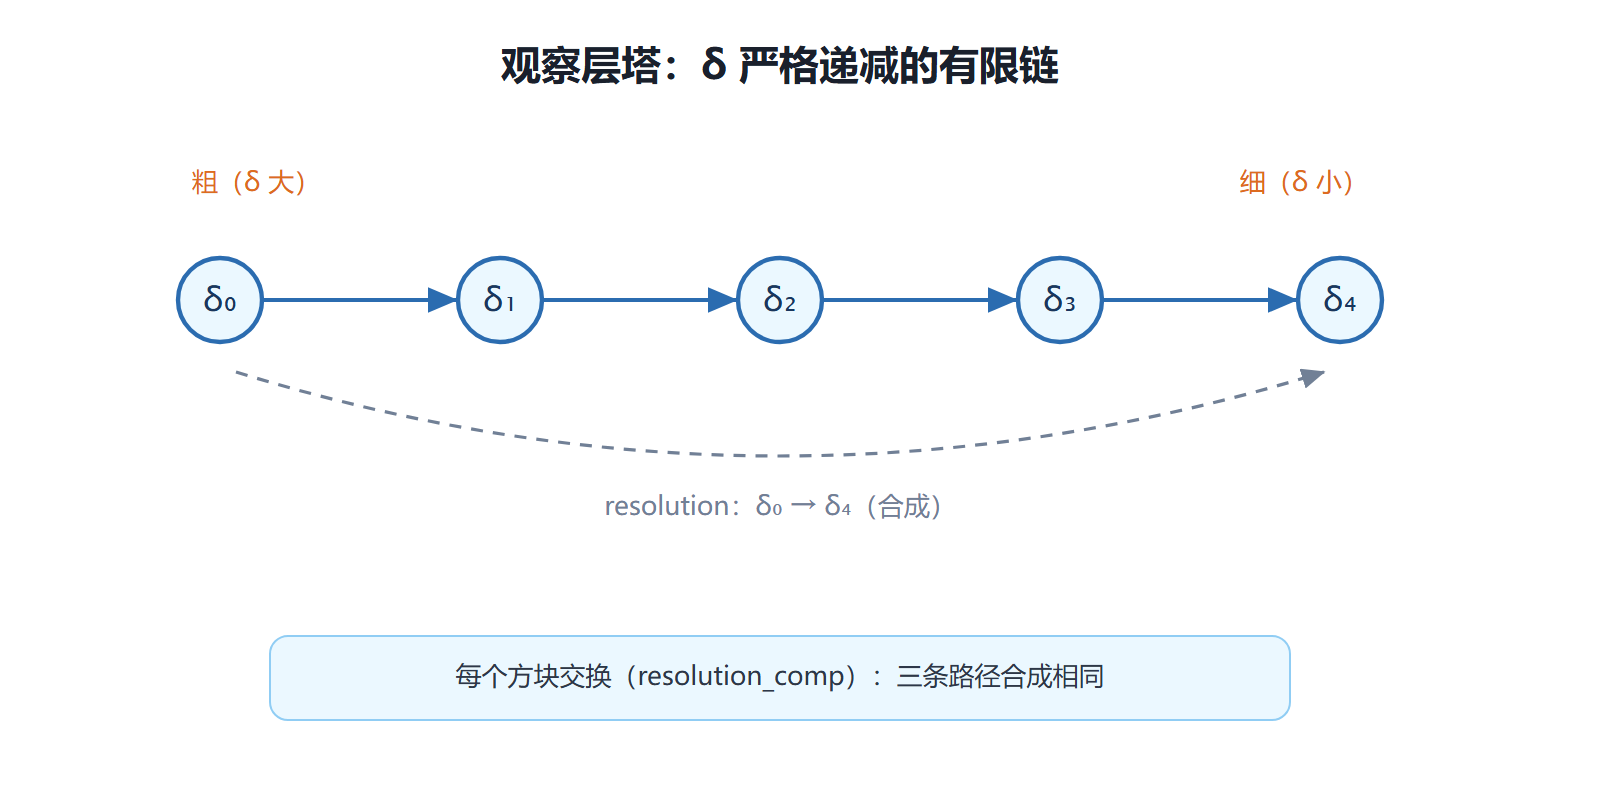
\includegraphics[width=0.92\textwidth]{figs/fig1_ladder.png}
\end{center}

\textbf{图 1.} 观察层塔的结构。节点是层（不同的分辨率 \texttt{\ensuremath{\\delta_{i}}}），箭头是消解（分辨率重采样）。虚线表示可复合的长程消解 \texttt{\ensuremath{\\delta_{0}} \ensuremath{\to} \ensuremath{\\delta_{4}}}。底部的方框是本文能在层塔上证明的唯一结构性事实：\textbf{每个方块都交换}——这正是 §8 中 \texttt{\ensuremath{b_{1}} \ensuremath{\equiv} 0} 的来源。

\textbf{为什么是有限链？}

三个理由：

\begin{enumerate}
\item \textbf{A1（有限）}：§2.1 的洞需要有限性才能计数；
\item \textbf{有序}：层的"优先级"就是 \texttt{\ensuremath{\delta}} 的序（§3 详述）；
\item \textbf{一维}：多层参数会立刻跌入不可分解（见 §3 的讨论）。
\end{enumerate}

\textbf{定义 2.10（凝结）.} 在层 \texttt{\ensuremath{\delta}} 下，两个状态"同层"如果它们的差异不超过 \texttt{\ensuremath{\delta}}：

\begin{lstlisting}
def ResLayer.indistinguishable (L : ResLayer) (x y : StateQuant n) : Prop :=
  commonDist x y ≤ L.δ
\end{lstlisting}

\textbf{但"不可区分"不传递}——\texttt{D(x,y) \ensuremath{\le} \ensuremath{\delta}} 且 \texttt{D(y,z) \ensuremath{\le} \ensuremath{\delta}} 不蕴含 \texttt{D(x,z) \ensuremath{\le} \ensuremath{\delta}}。

所以要取传递闭包：

\begin{lstlisting}
def ResLayer.related (L : ResLayer) (x y : StateQuant n) : Prop :=
  Relation.ReflTransGen (ResLayer.indistinguishable L) x y
\end{lstlisting}

\textbf{定理 2.11（同层是等价关系）.}

\begin{lstlisting}
theorem ResLayer.related_equivalence (L : ResLayer) :
    Equivalence (ResLayer.related L · ·)
\end{lstlisting}

于是可以取商：

\begin{lstlisting}
def ResLayer.condense (L : ResLayer) : Setoid (StateQuant n)
abbrev ResLayer.object (L : ResLayer) (n : ℕ) := Quotient (ResLayer.condense L)
\end{lstlisting}

\textbf{凝结对象就是"这一层看起来的一个点"。}

\subsection{消解是函子}

若 \texttt{\ensuremath{\\delta_{1}} \ensuremath{\le} \ensuremath{\\delta_{2}}}（\texttt{\ensuremath{\\delta_{2}}} 更粗），则粗层的每个对象都是细层对象的像：

\begin{lstlisting}
def ResLayer.resolution {δ₁ δ₂ : ℚ} (h : δ₁ ≤ δ₂) :
    ResLayer.object ⟨δ₁⟩ n → ResLayer.object ⟨δ₂⟩ n :=
  Quotient.map id (fun _ _ hxy => ResLayer.related_mono h hxy)
\end{lstlisting}

\textbf{定理 2.12（消解是函子）.}

\begin{lstlisting}
resolution (le_refl δ) = id
resolution h₂ ∘ resolution h₁ = resolution (h₁.trans h₂)
\end{lstlisting}

\begin{lstlisting}
theorem ResLayer.resolution_id (δ : ℚ) :
    ResLayer.resolution (le_refl δ) = id

theorem ResLayer.resolution_comp {δ₁ δ₂ δ₃ : ℚ} (h₁ : δ₁ ≤ δ₂) (h₂ : δ₂ ≤ δ₃)
    (q : ResLayer.object ⟨δ₁⟩ n) :
    ResLayer.resolution h₂ (ResLayer.resolution h₁ q) =
      ResLayer.resolution (h₁.trans h₂) q
\end{lstlisting}

\textbf{这两条是后文的全部支撑。}

\begin{itemize}
\item §4 的定义 4.3（相干）直接用了它们；
\item §5 的编码（\texttt{encode}）是它们的迭代；
\item §8 的"观察层塔无洞"（定理 8.1）就是它们的几何形式。
\end{itemize}

\textbf{换句话说：本文的层论之所以简单，是因为消解是函子。} 而消解是函子，是因为它只是"换分辨率"——同一个凝结对象的粗/细两种看法。

\bigskip

\section{紧层论：一个退化的 site}

\subsection{问题}

层论的威力来自一般性：site 可以是任意范畴配任意覆盖族，粘合公理于是成为一个\textbf{实质性的假设}——它要求：局部相容的数据总能唯一地拼成整体。

但一般性有代价：\textbf{粘合是否成立无法判定}。给定一个 site 和一族局部截面，判断它们能否粘合，一般需要计算上同调，而 \texttt{\ensuremath{H^{1}}} 通常不可计算。

本文的 site 极其特殊：

\begin{lstlisting}
structure LayerLadder where
  m : ℕ
  δ : Fin m → ℚ
  h_dec : ∀ i j, i < j → δ j < δ i
\end{lstlisting}

\textbf{一条有限、一维、严格递减的链。}

\textbf{本节要论证：在这条链上，粘合公理退化成定理。}

\subsection{覆盖只有一种}

在一般的 Grothendieck site 上，一个对象可以被\textbf{许多不同的覆盖族}覆盖。而在一维链上，一个层 \texttt{i} 只有两种"覆盖"：它自己，或者包含它的整条链。

\textbf{没有选择的余地，也就没有粘合问题。}

具体地，两个层 \texttt{i \ensuremath{\le} j} 之间只有一条路——\texttt{resolution}：

\begin{lstlisting}
def ResLayer.resolution {δ₁ δ₂ : ℚ} (h : δ₁ ≤ δ₂) :
    ResLayer.object ⟨δ₁⟩ n → ResLayer.object ⟨δ₂⟩ n
\end{lstlisting}

\textbf{"局部数据"在链上就是"某一层的对象"，"粘合"就是"往上消解"。}

\subsection{粘合公理变成定理}

\textbf{定理 3.1（全局截面 = 最细层）.}

\begin{lstlisting}
towerLimit L n  ≃  ResLayer.object ⟨δ_finest⟩ n
\end{lstlisting}

\begin{lstlisting}
theorem sheaf_topos_bridge (L : LayerLadder) (hm : 0 < L.m) (n : ℕ) :
    Nonempty (towerLimit L n ≃ ResLayer.object ⟨L.δ (L.finest hm)⟩ n)
\end{lstlisting}

其中 \texttt{towerLimit} 是相容族的集合（即 sheaf 的全局截面）：

\begin{lstlisting}
def towerLimit (L : LayerLadder) (n : ℕ) : Type :=
  { f : ∀ i : Fin L.m, ResLayer.object ⟨L.δ i⟩ n //
      ∀ i j (h : i ≤ j), ResLayer.resolution (L.le_delta h) (f j) = f i }
\end{lstlisting}

\textbf{这条定理说的正是}：在这条链上，粘合是\textbf{唯一且自动的}——任何最细层的对象都能向下消解成相容族，而任何相容族都由最细层唯一确定。

\textbf{粘合公理因此不是假设，是推论。}

\textbf{推论 3.2（相容族的构造）.}

\begin{lstlisting}
ladderToLimit  :  最细层对象  ⟶  相容族
limitToFinest  :  相容族      ⟶  最细层对象
\end{lstlisting}

且两者互逆（\texttt{ladderLimitEquiv}）。

\subsection{Mittag-Leffler 坍缩}

一般层论中，一个层塔的极限可能不等于任何一层——它可能"悬在中间"。Mittag-Leffler 条件正是排除这种病态的充分条件。

\textbf{定理 3.3（坍缩）.} 在有限链上，塔极限直接坍缩到最细层。

\begin{lstlisting}
theorem mittag_leffler_collapse (L : LayerLadder) (hm : 0 < L.m) (n : ℕ)
\end{lstlisting}

\textbf{这是定理 3.1 的另一面}：因为链是有限的，Mittag-Leffler 条件自动满足，所以极限不"悬空"，直接落到末端。

\subsection{代价：\ensuremath{H^{1}} = 0}

\textbf{一切都有代价。}

在一条链上，没有环，所以：

\textbf{定理 3.4.} 观察层塔的一个 2-胞腔恒交换：

\begin{lstlisting}
theorem layer_square_commutes (L : LayerLadder) (i j k : Fin L.m) :
    ResLayer.resolution (L.le_delta h₁) (ResLayer.resolution (L.le_delta h₂) q) =
      ResLayer.resolution (L.le_delta (h₁.trans h₂)) q
\end{lstlisting}

\textbackslash\{\}emph\{证明.\} 消解是函子（\texttt{resolution\_comp}）。

于是任何 2-胞腔都填满，\textbf{第一贝蒂数恒为 0}：

\begin{lstlisting}
b₁ = 1 − n² + 2n(n−1) − (n−1)² = 0
\end{lstlisting}

\textbf{更深的原因}：观察层塔对网络一无所知。

\textbf{定理 4.8（重述）.} 对任意端到端映射，按层塔观测得到的层族永远相干。

\begin{lstlisting}
Coherent L n (fun i => Quotient.mk ⟨δ_i⟩ (F x))
\end{lstlisting}

\textbf{所以 \texttt{\ensuremath{H^{1}} = 0} 不是网络的属性，是观测方式的属性。}

\textbf{这是"紧"的代价}：因为 site 太紧，上同调无处着力；因此任何基于 \texttt{\ensuremath{H^{1}}} 的诊断在观察层塔上都是空的。

§8 会说明：要承载诊断，必须把 sheaf 建在\textbf{计算图}上（层变换 \ensuremath{\times} 改述对），而不是观察层塔上。

\subsection{为什么仍然值得这么"紧"}

有三个理由。

\textbf{① 可计算性。}

一般的 \texttt{\ensuremath{H^{1}}} 不可计算。而在有限链上，一切都能写成显式公式：\texttt{\ensuremath{b_{1}} = 1 \ensuremath{-} V + E \ensuremath{-} F}，其中 \texttt{F} 是填满的面数。§8 正是靠这个把 \texttt{\ensuremath{b_{1}}} 算出来的。

\textbf{② 判据的存在。}

如果 site 是一般的，那么"障碍"到处都是——你无法区分哪个障碍来自网络结构，哪个只是 site 本身的性质。

\textbf{而在链上，唯一可能的障碍被隔离在一个明确的位置}：§4 的 \texttt{Coherent} 判据。它测的不是上同调，而是"层族能否由单源生成"。

\textbf{③ 有限性（A1）。}

§2.1 的洞需要有限才能计数。链的每条边、每个面都有限，所以整条链上的所有量都是可数的。

\textbf{这就是"紧层论"的含义}：不是放弃了层论，是把 site 压到一条链上，于是层论的机器全部塌缩成有限组合算术。

\subsection{与一般层论的关系一览}

\begin{center}\small
\begin{tabular}{lll}
\toprule
 & 一般 Grothendieck site & 本文的有限链 \\
\midrule
覆盖 & 任意覆盖族 & 只有一种 \\
粘合公理 & \textbf{假设} & \textbf{定理}（定理 3.1） \\
\texttt{\ensuremath{H^{1}}} & 可能非零、不可算 & \textbf{恒为 0}，可算 \\
极限 & 可能悬空 & \textbf{坍缩到末端}（定理 3.3） \\
诊断 & 靠上同调 & 靠 \texttt{Coherent}（§4） \\
\bottomrule
\end{tabular}
\end{center}

\bigskip

\section{可解释性判据}

\subsection{问题的形状}

我们想知道：一个神经网络的某一层，能不能被更浅的层解释？

这个问题的常见说法是"深层是不是浅层的某种可逆变换"。但"可逆"太强——大多数网络不可逆；"变换"太模糊——哪个变换？

§2 和 §3 已经搭好了框架：层塔是有限、一维、严格递减的序；每层有一个凝结（距离阈值的传递闭包）；相邻层之间有消解 \texttt{resolution}。

问题于是变成：

\begin{quote}
\textbf{一个网络态（每层一个凝结对象）什么时候是"自洽"的？}
\end{quote}

\subsection{网络是什么}

\textbf{这是本节最容易被跳过、却最重要的一步。}

先说清楚一件事：

\textbf{如果网络被建模成单个端到端映射} \texttt{F : StateQuant n \ensuremath{\to} StateQuant n}，那么按层塔观测得到的层族

\begin{lstlisting}
x  ↦  fun i => Quotient.mk ⟨δ_i⟩ (F x)
\end{lstlisting}

\textbf{永远相干}（定理 4.8）。证明只有一行。

所以必须在建模阶段就说清楚：\textbf{每层用的是不同的映射。}

\textbf{定义 4.1（网络）.} 一个网络由三部分组成：

\begin{itemize}
\item 一个层塔 \texttt{L}（有限、一维、严格递减）；
\item 一个\textbf{逐层映射族} \texttt{fs : Fin L.m \ensuremath{\to} (StateQuant n \ensuremath{\to} StateQuant n)}；
\item 层 \texttt{i} 的激活是 \texttt{fs i x}（对输入 \texttt{x}）。
\end{itemize}

\textbf{定义 4.2（网络态）.} 给定输入 \texttt{x}，网络态是每层的激活凝结到该层：

\begin{lstlisting}
def layerState (L : LayerLadder)
    (fs : Fin L.m → (StateQuant n → StateQuant n)) (x : StateQuant n) : NetState L n :=
  fun i => Quotient.mk (ResLayer.condense ⟨L.δ i⟩) (fs i x)
\end{lstlisting}

\textbf{这个区分不是技术细节。} 定理 4.8 会说明：不做这个区分，判据就是空的。

\subsection{相干性}

\textbf{定义 4.3（相干）.} 网络态 \texttt{f} 相干，如果粗层是细层的消解像：

\begin{lstlisting}
Coherent L n f  :=  ∀ i ≤ j,  resolution (i←j) (f j) = f i
\end{lstlisting}

\begin{lstlisting}
def Coherent (L : LayerLadder) (n : ℕ) (f : NetState L n) : Prop :=
  ∀ (i j : Fin L.m) (h : i ≤ j), ResLayer.resolution (L.le_delta h) (f j) = f i
\end{lstlisting}

直觉：\textbf{深层（粗层）不应该携带超出消解的新信息。}

\subsection{主判据}

记 \texttt{finest} 为最细层的索引（\texttt{\ensuremath{\delta}} 最小的那层）。

\textbf{定理 4.4（可解释 \ensuremath{\Longleftrightarrow} 由输入层决定）.}

\begin{lstlisting}
Coherent L n f  ⟺  ∃ g,  ∀ i,  f i = resolution (i←finest) g
\end{lstlisting}

\begin{lstlisting}
theorem interpretability_criterion (L : LayerLadder) (hm : 0 < L.m) (n : ℕ) :
    (∀ f : NetState L n, Coherent L n f ↔
      ∃ g : ResLayer.object ⟨L.δ (L.finest hm)⟩ n,
        ∀ i, f i = ResLayer.resolution (L.le_delta (le_finest L hm i)) g) ∧
    Nonempty (towerLimit L n ≃ ResLayer.object ⟨L.δ (L.finest hm)⟩ n)
\end{lstlisting}

\textbackslash\{\}emph\{证明.\}

\begin{itemize}
\item （\ensuremath{\Longrightarrow}）取 \texttt{g := f finest}。由相干性，\texttt{f i = resolution (i\ensuremath{\leftarrow}finest) (f finest)}。
\item （\ensuremath{\Longleftarrow}）若 \texttt{f = encode g} 形，则任意两条路径都等于直接消解，因为消解是函子（\texttt{resolution\_comp}）。
\end{itemize}

\textbf{定理 4.4 是本节的核心}：可解释性有一个\textbf{单源刻画}——整条层族由一个对象决定。

§5 会把这句话翻成更强的形式（编码 + 唯一性）。

\subsection{相干性的距离刻画}

定理 4.4 是结构性的，但不好直接检验。下面把它展开成距离条件。

\textbf{定理 4.5（相干 \ensuremath{\Longleftrightarrow} 逐层同层）.}

\begin{lstlisting}
Coherent L n (layerState L fs x)
  ⟺  ∀ i ≤ j,  ResLayer.related ⟨δ_i⟩ (fs j x) (fs i x)
\end{lstlisting}

\begin{lstlisting}
theorem layerState_coherent_iff (L : LayerLadder)
    (fs : Fin L.m → StateQuant n → StateQuant n) (x : StateQuant n) :
    Coherent L n (layerState L fs x) ↔
      ∀ (i j : Fin L.m), i ≤ j → ResLayer.related ⟨L.δ i⟩ (fs j x) (fs i x)
\end{lstlisting}

\textbackslash\{\}emph\{证明.\} 把 \texttt{Coherent} 展开：\texttt{resolution (i\ensuremath{\leftarrow}j) (Quotient.mk \ensuremath{\langle}\ensuremath{\delta}\_j\ensuremath{\rangle} y) = Quotient.mk \ensuremath{\langle}\ensuremath{\delta}\_i\ensuremath{\rangle} y}（由 \texttt{resolution\_condense}）。于是等式变成

\begin{lstlisting}
Quotient.mk ⟨δ_i⟩ (fs j x) = Quotient.mk ⟨δ_i⟩ (fs i x)
\end{lstlisting}

而这正是 \texttt{related \ensuremath{\langle}\ensuremath{\delta}\_i\ensuremath{\rangle} (fs j x) (fs i x)}（由商的相等性）。

\textbf{推论 4.6（充分条件）.}

\begin{lstlisting}
∀ i ≤ j,  commonDist (fs j x) (fs i x) ≤ δ_i   ⟹   Coherent L n (layerState L fs x)
\end{lstlisting}

\begin{lstlisting}
theorem layerState_coherent_of_close (L : LayerLadder)
    (h : ∀ i j, i ≤ j → commonDist (fs j x) (fs i x) ≤ L.δ i) :
    Coherent L n (layerState L fs x)
\end{lstlisting}

因为 \texttt{related} 由 \texttt{commonDist \ensuremath{\le} \ensuremath{\delta}} 生成（单步）。

\textbf{推论 4.6 是 §5 和 §6 的接口}：它把结构判据翻译成了距离判据，而距离正是 §6 的 gap 所使用的。

\textbf{推论 4.7（不相干的见证）.}

\begin{lstlisting}
¬ Coherent  ⟹  ∃ i ≤ j,  ¬ related ⟨δ_i⟩ (fs j x) (fs i x)
\end{lstlisting}

\begin{lstlisting}
theorem layerState_incoherent_witness (h : ¬ Coherent L n (layerState L fs x)) :
    ∃ (i j : Fin L.m), i ≤ j ∧ ¬ ResLayer.related ⟨L.δ i⟩ (fs j x) (fs i x)
\end{lstlisting}

\textbf{黑箱在层族层面有一个具体的地址}：不是"说不清"，是"这一对层对不上"。

\subsection{一个负面定理：为什么必须逐层}

现在兑现 4.2 的承诺。

\textbf{定理 4.8（单映射观测永远相干）.} 对\textbf{任意}端到端映射 \texttt{F} 和\textbf{任意}输入 \texttt{x}，

\begin{lstlisting}
Coherent L n (fun i => Quotient.mk ⟨δ_i⟩ (F x))
\end{lstlisting}

\begin{lstlisting}
theorem observation_always_coherent (L : LayerLadder)
    (F : StateQuant n → StateQuant n) (x : StateQuant n) :
    Coherent L n (fun i => Quotient.mk (ResLayer.condense ⟨L.δ i⟩) (F x))
\end{lstlisting}

\textbackslash\{\}emph\{证明.\} 每层都是\textbf{同一个值}的像；而 \texttt{resolution} 恰好是"同一个值换分辨率"，所以两条路径相等。

\textbf{这个定理的含义是：\texttt{Coherent} 单独不携带任何关于网络的信息。}

它的全部内容在"每层用的是\textbf{不同}的映射"这句话里——而这句话此前一直藏在我们对"网络"的默会理解中，没有被写下来。

\textbf{这不是技术细节，是模型的前提。}

\subsection{第二个判据：坍缩}

上面的判据是\textbf{结构}的（层族是否自洽）。还有一个\textbf{定量}的判据，关于单个映射丢了多少信息。

\textbf{定义 4.9（相干映射）.}

\begin{lstlisting}
CoherentMap δ F  :=  ∀ x y,  F x = F y → commonDist x y ≤ δ
\end{lstlisting}

\begin{lstlisting}
def CoherentMap (δ : ℚ) (f : StateQuant n → StateQuant m) : Prop :=
  ∀ x y, f x = f y → commonDist x y ≤ δ
\end{lstlisting}

直觉：\textbf{如果 \texttt{F} 把远处的点映到一起，它就破相干。}

\textbf{定理 4.10（恒等相干，ReLU 不相干）.}

\begin{lstlisting}
id 在任意 δ ≥ 0 下相干；ReLU 在任何 δ 下都不相干。
\end{lstlisting}

\begin{lstlisting}
theorem id_coherent (hδ : 0 ≤ δ) : CoherentMap δ (id : StateQuant n → StateQuant n)

theorem relu_gap_unbounded (δ : ℚ) :
    ¬ CoherentMap δ (reluState : StateQuant 1 → StateQuant 1)
\end{lstlisting}

\textbf{定理 4.11（可解释性刻度）.} \texttt{gap} 取遍 \texttt{[0, \ensuremath{\infty}]}：恒等在 0，ReLU 在 \ensuremath{\infty}。

\begin{lstlisting}
theorem interpretability_scale
\end{lstlisting}

这给出了一个有刻度的连续量——而不是"可解释/不可解释"的二值判断。

\textbf{定理 4.12（黑箱不可修复）.} 不相干在左复合下保持：

\begin{lstlisting}
¬ CoherentMap δ f   ⟹   ¬ CoherentMap δ (g ∘ f)
\end{lstlisting}

\begin{lstlisting}
theorem gap_compose_left (hf : ¬ CoherentMap δ f) :
    ¬ CoherentMap δ (fun x => g (f x))
\end{lstlisting}

\textbackslash\{\}emph\{证明.\} 若 \texttt{f} 把远处的 \texttt{x, y} 映到同一处，则 \texttt{g \ensuremath{\circ} f} 也把这两点映到同一处。\textbf{后续层只能在已有的等价类内部操作，无法把它们重新分开。}

\textbf{这是本节最重要的负面结论}：黑箱的深度是单调的。一旦某个位置切断了相干性，网络之后的所有层都建立在这个切口之上。

写成复合链的形式（CNN 的典型结构）：

\begin{lstlisting}
theorem cnn_gap_persists
\end{lstlisting}

\subsection{两条判据的分工}

现在可以清楚地说：本节给了两个判据，它们\textbf{不能互相推出}。

\begin{center}\small
\begin{tabular}{lll}
\toprule
 & \texttt{Coherent}（结构） & \texttt{CoherentMap}（定量） \\
\midrule
问的是 & 整条链能否由一个源生成 & 这一层丢了多少信息 \\
方向 & 存在源 \ensuremath{\Longrightarrow} 每层是源的像 & 相同输出 \ensuremath{\Longrightarrow} 输入近 \\
输出 & 真 / 假 & \texttt{\ensuremath{\delta} \ensuremath{\in} [0, \ensuremath{\infty}]} \\
后续 & §5（编码） & §6（gap） \\
\bottomrule
\end{tabular}
\end{center}

\textbf{为什么不能互推？}

\texttt{CoherentMap} 说的是"相同输出 \ensuremath{\Longrightarrow} 输入近"；它\textbf{不}给出"输入近 \ensuremath{\Longrightarrow} 输出近"。这个不对称有后果：定理 4.12 只在\textbf{否命题}方向成立。

\textbf{一个具体的对比}：一个网络可以每层都损失很大（\texttt{gap} 大）却仍然相干（每层都是同一个源的像）；也可以每层都无损（\texttt{gap = 0}）却不相干（各层来自不同的源）。

\textbf{前者是"压缩得厉害"，后者是"在说谎"。这两种是不同的问题。}

\subsection{小结}

本节建立了两个判据：

\begin{enumerate}
\item \textbf{结构判据}：\texttt{Coherent} \ensuremath{\Longleftrightarrow} 由输入层唯一决定（定理 4.4），且有距离刻画（定理 4.5）。
\item \textbf{定量判据}：\texttt{CoherentMap} 给出 \texttt{gap \ensuremath{\in} [0,\ensuremath{\infty}]}（定理 4.11），且黑箱不可修复（定理 4.12）。
\end{enumerate}

两者的分工（§4.8）是后面两节的分工：

\begin{itemize}
\item \textbf{§5} 把结构判据翻成编码：定理 4.4 的"存在源"变成"存在唯一、可逆的代码"。
\item \textbf{§6} 把定量判据算出数值：定理 4.11 的 \texttt{gap \ensuremath{\in} [0,\ensuremath{\infty}]} 在 ReLU 族上等于 \texttt{(c/a+1)²}。
\end{itemize}

\bigskip

\section{主定理：可解释性 = 可编码性}

\subsection{从否定式到肯定式}

§4 给出的判据是\textbf{否定式}的：

\begin{quote}
一个网络可解释，当且仅当它的深层不携带超出消解的新信息。
\end{quote}

这个说法精确，但不好用。它告诉你不该有什么，没告诉你该有什么。要检验一个网络，你得逐层检查"有没有新东西"——这是一个\textbf{全称命题的否定}，在实践中无法穷尽。

本节把它翻成\textbf{肯定式}：

\begin{quote}
一个网络可解释，当且仅当\textbf{存在一个对象，它编码了整条层族}。
\end{quote}

这不是修辞层面的改写。否定式是\textbf{约束}，肯定式是\textbf{构造}。有构造就能算，有约束只能查。

\subsection{编码与解码}

设 \texttt{L} 是层塔，\texttt{n} 是维度，\texttt{f : NetState L n} 是网络态——每层一个凝结对象：

\begin{lstlisting}
def NetState (L : LayerLadder) (n : ℕ) : Type :=
  ∀ i : Fin L.m, ResLayer.object ⟨L.δ i⟩ n
\end{lstlisting}

两个基本操作：

\textbf{定义 5.1（解码）.} 取最细层的那个对象。

\begin{lstlisting}
def decode (L : LayerLadder) (hm : 0 < L.m) (f : NetState L n) :
    ResLayer.object ⟨L.δ (L.finest hm)⟩ n :=
  f (L.finest hm)
\end{lstlisting}

\textbf{定义 5.2（编码）.} 把唯一的源沿塔逐层消解，重建整条层族。

\begin{lstlisting}
def encode (L : LayerLadder) (hm : 0 < L.m)
    (g : ResLayer.object ⟨L.δ (L.finest hm)⟩ n) : NetState L n :=
  fun i => ResLayer.resolution (L.le_delta (le_finest L hm i)) g
\end{lstlisting}

注意：\textbf{两个定义都不依赖任何假设}。它们对任意网络态、任意层对象都有定义。区别只在于它们是否互逆。

\subsection{编解码互逆}

\textbf{定理 5.3（解码再编码 = 恒等）.} 对任意源 \texttt{g}，

\begin{lstlisting}
decode L hm (encode L hm g) = g
\end{lstlisting}

\textbackslash\{\}emph\{证明.\} 取最细层时消解是恒等。形式化为 \texttt{resolution\_self}：对任意 \texttt{h : \ensuremath{\delta} \ensuremath{\le} \ensuremath{\delta}}，\texttt{resolution h q = q}（由恒等消解 \texttt{resolution\_refl} 与证明无关性得到）。

\begin{lstlisting}
theorem resolution_self {δ : ℚ} (h : δ ≤ δ) (q : ResLayer.object ⟨δ⟩ n) :
    ResLayer.resolution h q = q := by
  rw [show h = le_refl δ from Subsingleton.elim h _]
  exact resolution_refl q
\end{lstlisting}

\textbf{定理 5.4（编码再解码 = 恒等，相干时）.} 若 \texttt{f} 相干，则

\begin{lstlisting}
encode L hm (decode L hm f) = f
\end{lstlisting}

\textbackslash\{\}emph\{证明.\} 相干性给出 \texttt{f} 完全由它在最细层的值决定（\texttt{coherent\_has\_source}）；而 \texttt{encode} 是函数性的，所以重建出的层族逐层相等。

\textbf{推论 5.5（编码单射）.} \texttt{encode} 是单射：不同的源给出不同的层族。

\begin{lstlisting}
theorem encode_injective (L : LayerLadder) (hm : 0 < L.m) :
    Function.Injective (encode L hm (n := n))
\end{lstlisting}

\textbackslash\{\}emph\{证明.\} 若 \texttt{encode g = encode g'}，取最细层并应用定理 5.3 即得 \texttt{g = g'}。

\textbf{于是：相干网络态与单层对象之间是一一对应。} 这就是"可编码"的精确含义——不是模糊的"能被理解"，而是"被一个具体的、唯一的对象生成"。

\begin{center}
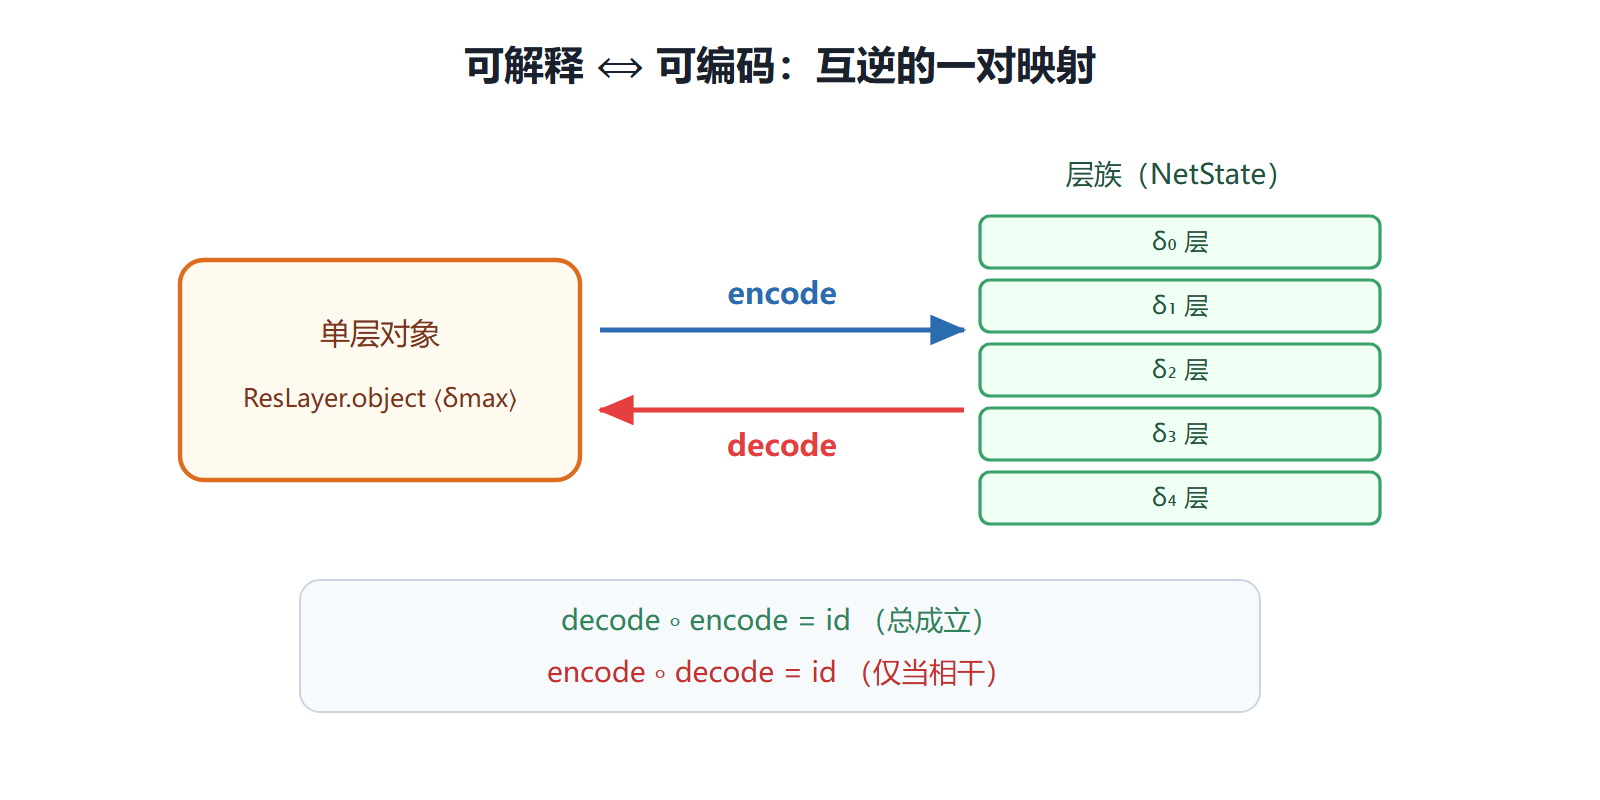
\includegraphics[width=0.92\textwidth]{figs/fig2_encode.png}
\end{center}

\textbf{图 2.} 编码与解码是一对互逆映射。注意两个方向的不对称性：\texttt{decode \ensuremath{\circ} encode = id} 对\textbf{任何}源都成立（定理 5.3），而 \texttt{encode \ensuremath{\circ} decode = id} 只在层族相干时成立（定理 5.4）。\textbf{这个不对称正是"可解释性"的判据}——相干就是回到原点。

\subsection{主定理}

\textbf{定理 5.6（可解释 = 可编码）.}

\begin{lstlisting}
Coherent L n f  ⟺  ∃ g, f = encode L hm g
\end{lstlisting}

\textbackslash\{\}emph\{证明.\}

\begin{itemize}
\item （\ensuremath{\Longrightarrow}）取 \texttt{g := decode L hm f}，由定理 5.4 得 \texttt{f = encode (decode f)}。
\item （\ensuremath{\Longleftarrow}）编码总是相干的（定理 5.7）。
\end{itemize}

\begin{lstlisting}
theorem interpretability_is_encodability (L : LayerLadder) (hm : 0 < L.m) (n : ℕ) :
    (∀ f : NetState L n, Coherent L n f ↔ ∃ g, f = encode L hm g) ∧
    (∀ g, Coherent L n (encode L hm g)) ∧
    Function.Injective (encode L hm) ∧
    (∀ g, decode L hm (encode L hm g) = g) ∧
    (∀ f, Coherent L n f → encode L hm (decode L hm f) = f)
\end{lstlisting}

\textbf{定理 5.7（编码总是相干）.}

\begin{lstlisting}
∀ g,  Coherent L n (encode L hm g)
\end{lstlisting}

\textbackslash\{\}emph\{证明.\} 编码由沿塔消解生成；任意两条路径都等于直接消解，因为消解是函子（\texttt{resolution\_comp}）。

\begin{lstlisting}
theorem layer_square_commutes (L : LayerLadder) (i j k : Fin L.m)
    (h₁ : i ≤ j) (h₂ : j ≤ k) :
    resolution (le_delta h₁) (resolution (le_delta h₂) q) =
      resolution (le_delta (h₁.trans h₂)) q
\end{lstlisting}

\textbf{这是全文的核心命题。} 可解释性有一个\textbf{对象级}的等价刻画：不是"没有新信息"（否定），而是"有一个源"（存在）。

\subsection{黑箱的肯定式定义}

\textbf{推论 5.8（黑箱 = 没有代码）.}

\begin{lstlisting}
¬ Coherent L n f   ⟹   ¬ ∃ g,  f = encode L hm g
\end{lstlisting}

\begin{lstlisting}
theorem incoherent_not_encodable (L : LayerLadder) (hm : 0 < L.m)
    (h : ¬ Coherent L n f) : ¬ ∃ g, f = encode L hm g
\end{lstlisting}

这不是把否定式换了个说法。它给出了黑箱的一个\textbf{存在性否定}：

\begin{quote}
\textbf{不存在能生成它的源。}
\end{quote}

而这比"说明不了"强得多——它在原则上是可检验的：\textbf{只要穷举所有源，就能确认它是黑箱。} 诚然源的全体可能很大，但它是\textbf{确定的}，不是"我们不知道"。

（§8 会给出这个"不存在"的拓扑对应物：非零的第一贝蒂数。）

\subsection{与映射判据的关系：为什么是两个判据}

必须诚实交代：本节的可编码性判据，\textbf{不能}由 §4 的映射判据（\texttt{CoherentMap}）推出，反之亦然。

\begin{lstlisting}
CoherentMap δ F  :=  ∀ x y, F x = F y → commonDist x y ≤ δ
\end{lstlisting}

两者不能互推，对照表和解剖见 §4.8（那里是首次提出）。本节只补一点这个不对称对\textbf{编码}意味着什么：

\begin{itemize}
\item \texttt{Coherent} 的失败是\textbf{"没有代码"}——不存在单个源能复现整条链；
\item \texttt{CoherentMap} 的失败是\textbf{"代码不是单射"}——码存在，但同一个码字对应了太多原文（\texttt{gap} 大）。
\end{itemize}

\textbf{前者：编码不存在。后者：编码不唯一。} 这是两种完全不同的坏法，§6 给后者的精确量化。

\subsection{一个必须交代的前提}

本节的全部结论依赖一个建模选择：\textbf{网络必须是逐层映射族}（定义 4.1）。

理由见 §4.6：如果网络被建模成单个端到端映射并按层塔观测，得到的层族\textbf{永远相干}（定理 4.8）——那样 \texttt{Coherent} 就是恒真的空命题。

而在逐层模型下，\texttt{Coherent} 有精确的距离刻画（定理 4.5）：

\begin{lstlisting}
Coherent L n (layerState L fs x)
  ⟺  ∀ i ≤ j,  ResLayer.related ⟨L.δ i⟩ (fs j x) (fs i x)
\end{lstlisting}

\textbf{这把结构判据翻译成了距离判据}（推论 4.6），而距离正是 §6 的 gap 所使用的。

所以：§4 的判据、§5 的编码、§6 的 gap 三条线，在这一点上接上了同一张网。

\subsection{小结}

本节建立了三件事：

\begin{enumerate}
\item \textbf{编码存在}：相干网络态 ⟷ 单层对象（定理 5.6 + 推论 5.5）。
\item \textbf{编码唯一}：编解码互逆，因此"代码"是确定的（定理 5.3、5.4）。
\item \textbf{黑箱有定义}：不相干 \ensuremath{\Longleftrightarrow} 无源（推论 5.8）。
\end{enumerate}

而支撑这些的是一个\textbf{结构事实}：消解是函子（定理 5.7），所以编码出来的层族必然自洽。

\textbf{最后的建模前提（§5.7，依据定理 4.8）} 则说明：层塔判据之所以有意义，是因为网络被写成逐层映射族；写成单个端到端映射时，判据会退化为恒真的空命题。

\bigskip

\section{gap 的精确值}

\textbf{本节的范围。} §6 只做一件事：把 \texttt{gap} 算出来。单层的闭式（6.3）、两层塌成一层（6.5）、复合律（6.6）、四条推论（6.7）。\textbf{这只是"代价是多少"。}

"代价意味着什么"——它和泛化、容量、鲁棒性的关系——在 §7，可以独立阅读。

\subsection{为什么 ReLU 的 gap 是 \ensuremath{\infty}}

§4 说 \texttt{gap \ensuremath{\in} [0, \ensuremath{\infty}]}：恒等映射在 0，ReLU 在 \ensuremath{\infty}。

但 ReLU 之所以是 \ensuremath{\infty}，\textbf{不是因为它坏，是因为定义域无界}。

\texttt{CoherentMap \ensuremath{\delta} F} 要求：只要 \texttt{F x = F y}，就有 \texttt{commonDist x y \ensuremath{\le} \ensuremath{\delta}}。而 ReLU 把整个负半轴压成 0——取 \texttt{x = 0}、\texttt{y = \ensuremath{-}t}，无论 \texttt{t} 多大都有 \texttt{F x = F y}。于是任何有限的 \texttt{\ensuremath{\delta}} 都不够。

\textbf{所以正确的问题不是"gap 是不是有限"，而是：}

\begin{quote}
\textbf{在一个有界的输入域上，它是多少？}
\end{quote}

这个问题在实践中有意义——真实网络的输入几乎总被归一化到有界盒（LayerNorm、tanh 饱和、或显式的归一化）。

\subsection{定义}

\textbf{定义 6.1（有界域上的相干）.} 设 \texttt{f : \ensuremath{\mathbb{Q}} \ensuremath{\to} \ensuremath{\mathbb{Q}}}，\texttt{B > 0}。

\begin{lstlisting}
CoherentOnBox B δ f  :=  ∀ x y,  |x| ≤ B → |y| ≤ B → f x = f y → (x − y)² ≤ δ
\end{lstlisting}

\begin{lstlisting}
def CoherentOnBox (B δ : ℚ) (f : ℚ → ℚ) : Prop :=
  ∀ x y : ℚ, |x| ≤ B → |y| ≤ B → f x = f y → (x - y) ^ 2 ≤ δ
\end{lstlisting}

\textbf{定义 6.2（gap）.} \texttt{g} 是 \texttt{f} 在盒 \texttt{B} 上的 gap，如果它是相干阈值且最小：

\begin{lstlisting}
IsGap B f g  :=  CoherentOnBox B g f  ∧  ∀ δ, CoherentOnBox B δ f → g ≤ δ
\end{lstlisting}

\begin{lstlisting}
def IsGap (B : ℚ) (f : ℚ → ℚ) (g : ℚ) : Prop :=
  CoherentOnBox B g f ∧ ∀ δ : ℚ, CoherentOnBox B δ f → g ≤ δ
\end{lstlisting}

\textbf{为什么用关系而不是函数？} 因为 \ensuremath{\mathbb{Q}} 没有良序，"最小的 \texttt{\ensuremath{\delta}}"不能直接写成 \texttt{sInf}。把"\texttt{g} 是 gap"写成关系，既精确又构造。

于是"gap = \texttt{(c/a+1)²}"被精确陈述为 \texttt{IsGap 1 (reluAffine a c) ((c/a+1)²)}。

\subsection{单层的精确值}

取最简的具体网络：

\begin{lstlisting}
f(x) = max 0 (a·x − c),   x ∈ [−1, 1],   a > 0, 0 ≤ c ≤ a
\end{lstlisting}

\textbf{坍缩集}是 \texttt{\{x : a\ensuremath{\cdot}x \ensuremath{-} c \ensuremath{\le} 0\} = \{x \ensuremath{\le} c/a\}}（因为 \texttt{a > 0}）。

所以最远的一对被压在一起：\textbf{\texttt{x = \ensuremath{-}1} 与 \texttt{y = c/a}}。

\begin{lstlisting}
距离 = (c/a − (−1))² = (c/a + 1)²
\end{lstlisting}

\textbf{定理 6.3（上界）.}

\begin{lstlisting}
∀ x y ∈ [−1,1],  f x = f y  ⟹  (x − y)² ≤ (c/a + 1)²
\end{lstlisting}

\textbackslash\{\}emph\{证明.\} 分三种情形。

\begin{itemize}
\item \textbf{两者都不截断}（\texttt{a\ensuremath{\cdot}x \ensuremath{-} c > 0} 且 \texttt{a\ensuremath{\cdot}y \ensuremath{-} c > 0}）：此时 \texttt{f} 在该区域是线性的且严格单增（\texttt{a > 0}），故 \texttt{f x = f y} 蕴含 \texttt{x = y}，距离为 0。
\item \textbf{两者都截断}（\texttt{a\ensuremath{\cdot}x \ensuremath{-} c \ensuremath{\le} 0} 且 \texttt{a\ensuremath{\cdot}y \ensuremath{-} c \ensuremath{\le} 0}）：由 \texttt{a > 0} 得 \texttt{x, y \ensuremath{\le} c/a}；又都在 \texttt{[\ensuremath{-}1,1]} 内，故 \texttt{x \ensuremath{-} y \ensuremath{\in} [\ensuremath{-}(c/a+1), c/a+1]}，平方不超过 \texttt{(c/a+1)²}。
\item \textbf{一截断一不截断}：\textbf{这种情形不会发生。} 不妨设 \texttt{a\ensuremath{\cdot}x \ensuremath{-} c > 0} 而 \texttt{a\ensuremath{\cdot}y \ensuremath{-} c \ensuremath{\le} 0}。则 \texttt{f x = a\ensuremath{\cdot}x \ensuremath{-} c > 0} 而 \texttt{f y = 0}，于是 \texttt{f x \ensuremath{\ne} f y}，与假设矛盾。同理 \texttt{y} 截断 \texttt{x} 不截断时亦然。
\end{itemize}

\textbf{定理 6.4（紧性）.} 上界被达到。

\begin{lstlisting}
x = −1,  y = c/a   ⟹   f x = f y = 0,   (x − y)² = (c/a + 1)²
\end{lstlisting}

\begin{lstlisting}
theorem reluAffine_gap_exact (ha : 0 < a) (hc0 : 0 ≤ c) (hc : c ≤ a) :
    (∀ x y, -1 ≤ x → x ≤ 1 → -1 ≤ y → y ≤ 1 →
      reluAffine a c x = reluAffine a c y → (x - y) ^ 2 ≤ (c / a + 1) ^ 2) ∧
    (∃ x y, -1 ≤ x ∧ x ≤ 1 ∧ -1 ≤ y ∧ y ≤ 1 ∧
      reluAffine a c x = reluAffine a c y ∧ (x - y) ^ 2 = (c / a + 1) ^ 2)
\end{lstlisting}

\textbf{定理 6.5（精确值）.}

\begin{lstlisting}
gap(f, 1) = (c/a + 1)²
\end{lstlisting}

用定义 6.2 的 \texttt{IsGap} 精确陈述：

\begin{lstlisting}
theorem reluAffine_isGap (ha : 0 < a) (hc0 : 0 ≤ c) (hc : c ≤ a) :
    IsGap 1 (reluAffine a c) ((c / a + 1) ^ 2)
\end{lstlisting}

\textbackslash\{\}emph\{证明.\} 拆成两部分：\texttt{CoherentOnBox}（定理 6.3）与最小性——由定理 6.4 的见证对 \texttt{x = \ensuremath{-}1, y = c/a}，任何有效 \texttt{\ensuremath{\delta}} 都必须 \texttt{\ensuremath{\ge} (x\ensuremath{-}y)² = (c/a+1)²}。

\textbf{这就是"gap 的精确值"}：一个可以写下来的数。

（本节只算 \texttt{B = 1} 的情形。\texttt{B} 一般时结论的形式相同，只是阈值换成 \texttt{c/a + B}——我们不需要它，故不展开。）

\subsection{端点与单调}

\textbf{定理 6.6（两端点）.}

\begin{lstlisting}
c = 0  ⟹  gap = 1      （标准 ReLU：max 0 (a·x)）
c = a  ⟹  gap = 4      （ReLU 杀死整个输入盒）
\end{lstlisting}

\begin{lstlisting}
theorem reluAffine_isGap_zero (ha : 0 < a) : IsGap 1 (reluAffine a 0) 1
theorem reluAffine_isGap_full (ha : 0 < a) : IsGap 1 (reluAffine a a) 4
\end{lstlisting}

\textbf{第一个数字最重要：标准 ReLU 的 gap = 1，不是 0。}

它意味着：\textbf{任何 ReLU 层都至少损失 1 个单位的距离}——因为负半轴整段被压成 0，最远可跨 \texttt{\ensuremath{-}1} 到 \texttt{0}。

这与 §4 的"ReLU 破相干"完全吻合，但现在它有了一个具体的量：\textbf{它破掉了恰好 1 个单位。}

\textbf{定理 6.7（单调）.} \texttt{gap} 关于 \texttt{c/a} 单调递增。

\begin{lstlisting}
theorem reluAffine_gap_monotone (h1 : 0 ≤ c₁) (h12 : c₁ ≤ c₂) :
    (c₁ / a + 1) ^ 2 ≤ (c₂ / a + 1) ^ 2
\end{lstlisting}

所以：

\begin{center}\small
\begin{tabular}{lll}
\toprule
c/a & gap & 含义 \\
\midrule
0 & \textbf{1} & 标准 ReLU \\
1/2 & 9/4 &  \\
1 & \textbf{4} & 杀死整个输入盒 \\
\bottomrule
\end{tabular}
\end{center}

\textbf{gap 只依赖 bias / weight 之比。}

\begin{center}
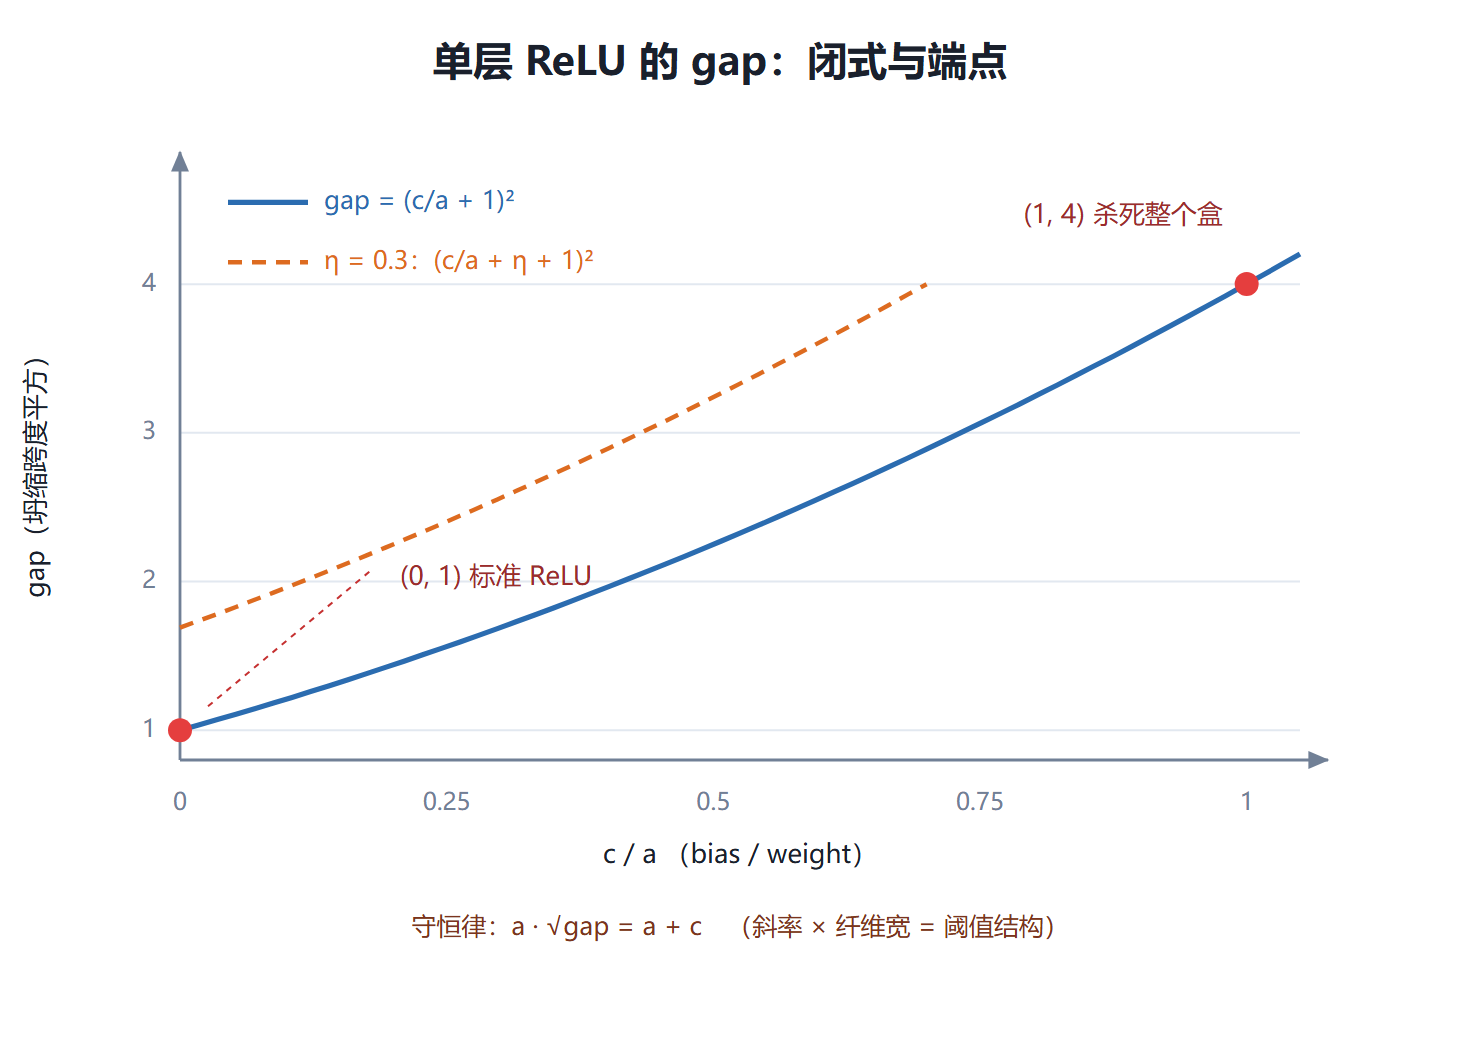
\includegraphics[width=0.92\textwidth]{figs/fig3_gap.png}
\end{center}

\textbf{图 3.} \texttt{gap} 关于 \texttt{c/a} 的闭式。两个端点就是定理 6.5 的整条内容：\texttt{c = 0} 给 1，\texttt{c = a} 给 4。\textbf{标准 ReLU 坐在 1 上，不是 0}——它一开始就付出了代价。虚线是 \ensuremath{\eta}-近似版本 \texttt{((c+\ensuremath{\eta})/a + 1)²}，两条曲线的纵向间距恒为 \texttt{\ensuremath{\eta}/a}（定理 7.9），这就是"近似可解释的汇率"。

\subsection{两层塌成一层}

要谈多层，先要一个结构事实。

\textbf{定理 6.8（一维两层 ReLU = 一层）.}

\begin{lstlisting}
max 0 (a₂ · max 0 (a₁x − c₁) − c₂) = max 0 (a₁a₂ · x − (a₂c₁ + c₂))
\end{lstlisting}

\begin{lstlisting}
theorem reluAffine2_eq_single (h2a : 0 < a₂) (h2c : 0 ≤ c₂) (x : ℚ) :
    reluAffine2 a₁ c₁ a₂ c₂ x = reluAffine (a₁ * a₂) (a₂ * c₁ + c₂) x
\end{lstlisting}

\textbackslash\{\}emph\{证明.\} 分两种情形。

\begin{itemize}
\item 内层未被截断（\texttt{\ensuremath{a_{1}}x \ensuremath{-} \ensuremath{c_{1}} > 0}）：两边都直接代入，\texttt{\ensuremath{a_{1}}\ensuremath{a_{2}}x \ensuremath{-} (\ensuremath{a_{2}}\ensuremath{c_{1}}+\ensuremath{c_{2}}) = \ensuremath{a_{2}}(\ensuremath{a_{1}}x \ensuremath{-} \ensuremath{c_{1}}) \ensuremath{-} \ensuremath{c_{2}}}。
\item 内层被截断（\texttt{\ensuremath{a_{1}}x \ensuremath{-} \ensuremath{c_{1}} \ensuremath{\le} 0}）：左边 \texttt{= max 0 (\ensuremath{-}\ensuremath{c_{2}}) = 0}；右边 \texttt{= max 0 (\ensuremath{a_{2}}(\ensuremath{a_{1}}x \ensuremath{-} \ensuremath{c_{1}}) \ensuremath{-} \ensuremath{c_{2}}) \ensuremath{\le} max 0 (\ensuremath{-}\ensuremath{c_{2}}) = 0}，又非负，故也是 0。
\end{itemize}

\textbf{注意：这里不需要 \texttt{\ensuremath{a_{1}} > 0}。} 一维 ReLU 在复合下塌缩成一个单层 ReLU——因为 ReLU 分段线性且\textbf{只有一个折点}，折点复合后仍然只有一个折点。

\subsection{复合律}

有了定理 6.8，两层的 gap 直接由 §6.3 给出：

\begin{lstlisting}
compThreshold := (c₁ + c₂/a₂) / a₁
gap(g∘f, 1) = (compThreshold + 1)²
\end{lstlisting}

\textbf{定理 6.9（两层 gap 的精确值）.}

\begin{lstlisting}
theorem gap_two_layer (ha : 0 < a₁) (hc1 : 0 ≤ c₁)
    (h2a : 0 < a₂) (h2c : 0 ≤ c₂) (h2c' : c₂ ≤ a₂ * (a₁ - c₁)) :
    (∀ x y ∈ [−1,1], reluAffine2 ... x = reluAffine2 ... y →
      (x - y) ^ 2 ≤ (compThreshold a₁ c₁ a₂ c₂ + 1) ^ 2) ∧
    (∃ x y, ... ∧ (x - y) ^ 2 = (compThreshold a₁ c₁ a₂ c₂ + 1) ^ 2)
\end{lstlisting}

把它和两层的 gap 对比，得到一个\textbf{非加非乘}的律：

\textbf{定理 6.10（复合律）.}

\begin{lstlisting}
√gap(g∘f) = √gap(f) + (√gap(g) − 1) / a₁
\end{lstlisting}

\begin{lstlisting}
theorem gap_compose_law (h1a : 0 < a₁) (h2a : 0 < a₂) :
    compThreshold a₁ c₁ a₂ c₂ + 1 = (c₁ / a₁ + 1) + ((c₂ / a₂ + 1) - 1) / a₁
\end{lstlisting}

其中 \texttt{\ensuremath{\sqrt{\mathrm{gap}}}(f) = \ensuremath{c_{1}}/\ensuremath{a_{1}} + 1}，\texttt{\ensuremath{\sqrt{\mathrm{gap}}}(g) = \ensuremath{c_{2}}/\ensuremath{a_{2}} + 1}。

\textbf{\texttt{\ensuremath{a_{1}} = 1} 时最干净：}

\begin{lstlisting}
√gap(g∘f) = √gap(f) + √gap(g) − 1
\end{lstlisting}

\textbf{为什么有个 \ensuremath{-}1？} 因为标准 ReLU 的 gap 是 \textbf{1} 而不是 0——两层的"1"只该算一次。

\textbf{这个 \ensuremath{-}1 就是定理 6.6 那个 1 的减法形式。} §6.4 和 §6.6 说的是同一件事。

\subsection{四条推论}

\textbf{推论 6.11（不可加）.} 两层标准 ReLU，每层 gap 都是 1，复合的 gap 还是 1，不是 4。

\begin{lstlisting}
theorem gap_not_additive :
    compThreshold 1 0 1 0 + 1 = 1 ∧ (1 : ℚ) ≠ (0 / 1 + 1) + (0 / 1 + 1)
\end{lstlisting}

\textbf{推论 6.12（幂等）.} \texttt{max 0 (max 0 x) = max 0 x}。

\begin{lstlisting}
theorem relu_compose_idempotent (x : ℚ) : reluAffine2 1 0 1 0 x = reluAffine 1 0 x
\end{lstlisting}

\textbf{推论 6.13（加层不减 gap）.} \texttt{\ensuremath{\sqrt{\mathrm{gap}}}(f) \ensuremath{\le} \ensuremath{\sqrt{\mathrm{gap}}}(g\ensuremath{\circ}f)}。

\begin{lstlisting}
theorem gap_depth_monotone (hc1 : 0 ≤ c₁) (hc2 : 0 ≤ c₂) :
    c₁ / a₁ + 1 ≤ compThreshold a₁ c₁ a₂ c₂ + 1
\end{lstlisting}

\textbf{推论 6.14（L 层闭式）.} 递归复合律：单位权重下 \texttt{\ensuremath{\sqrt{\mathrm{gap}}}\_L = 1 + \ensuremath{\Sigma} \ensuremath{c_{i}}}，即

\begin{lstlisting}
gap(L 层单位权重) = (1 + Σ cᵢ)²
\end{lstlisting}

\textbackslash\{\}emph\{证明.\} 反复使用定理 6.8（两层塌成一层），得 L 个 \texttt{reluAffine 1 \ensuremath{c_{i}}} 的复合等于单个 \texttt{reluAffine 1 (\ensuremath{\Sigma}\ensuremath{c_{i}})}；再套用定理 6.5。

\begin{lstlisting}
def reluIter : List ℚ → ℚ → ℚ
  | [], x => x
  | c :: cs, x => reluIter cs (reluAffine 1 c x)

theorem reluIter_eq_single (c₀ : ℚ) (cs : List ℚ)
    (hall : ∀ c ∈ c₀ :: cs, 0 ≤ c) :
    ∀ x : ℚ, reluIter (c₀ :: cs) x = reluAffine 1 (c₀ + cs.sum) x

theorem reluIter_isGap (cs : List ℚ) (hne : cs ≠ [])
    (h0 : ∀ c ∈ cs, 0 ≤ c) (h1 : cs.sum ≤ 1) :
    IsGap 1 (reluIter cs) ((cs.sum + 1) ^ 2)
\end{lstlisting}

\textbf{深度的代价是平方增长的。}

\subsection{讨论：gap 是什么指标}

\textbf{第一，gap 是可算的，不是定性的。}

给定一层 ReLU，它的"不可解释性"就是一个数：\texttt{(bias/weight + 1)²}。这与 §5.6 那句"这个网络压缩得厉害"对上了——\textbf{"厉害"现在是一个数。}

\textbf{第二，gap 是可归因的。}

复合律 \texttt{\ensuremath{\sqrt{\mathrm{gap}}}(g\ensuremath{\circ}f) = \ensuremath{\sqrt{\mathrm{gap}}}(f) + (\ensuremath{\sqrt{\mathrm{gap}}}(g) \ensuremath{-} 1)/\ensuremath{a_{1}}} 说明：每加一层，\texttt{\ensuremath{\sqrt{\mathrm{gap}}}} 增加 \texttt{(\ensuremath{\sqrt{\mathrm{gap}}}(新层) \ensuremath{-} 1)/\ensuremath{a_{1}}}。

\begin{itemize}
\item 标准 ReLU 的 \texttt{1} 是\textbf{免费额度}——第一层不额外收费；
\item 之后每层收 \texttt{\ensuremath{\sqrt{\mathrm{gap}}} \ensuremath{-} 1}；
\item \textbf{增益 \texttt{\ensuremath{a_{1}}} 越大，下一层的贡献越小}。
\end{itemize}

\textbf{第三，gap 与 §4 的"深度 = 切口数"吻合，但更细。}

§4 说深度是切口数。这里说：\textbf{不是每个切口同等收费，收费额是 \texttt{(\ensuremath{\sqrt{\mathrm{gap}}}(切口) \ensuremath{-} 1) / 增益}。}

\subsection{诚实的边界}

本节的全部结论都在 \textbf{1 维、有界盒、单层或两层} 上。

这不是一般的限制，是\textbf{刻意的起点}：

\begin{itemize}
\item 1 维：坍缩集是半轴，最远距离可以精确写出；
\item 有界：无界时 gap 恒为 \ensuremath{\infty}，见 §6.1；
\item 单层/两层：一维 ReLU 的折点只有一个，所以能塌成一层（定理 6.8）。
\end{itemize}

\textbf{三维及以上的一般情形，本文不做断言}——但有一个例外已经算清（§7.6）：整个盒坍缩时，\texttt{gap = 4n\ensuremath{B^{2}}}。而 §6.5 的结构定理提示了一般情形为什么难：\textbf{多维 ReLU 的坍缩集是半空间，复合后通常不再是单个半空间}——所以"塌成一层"在多维不成立，复合律也需要重写。

具体地说，设状态空间是 \texttt{\ensuremath{\mathbb{Q}}ⁿ} 的盒 \texttt{B}。一层 \texttt{x \ensuremath{\mapsto} ReLU(Wx \ensuremath{-} c)}（\texttt{W : \ensuremath{\mathbb{Q}}ⁿ \ensuremath{\to} \ensuremath{\mathbb{Q}}}）的坍缩集是半空间与盒的交：

\begin{lstlisting}
C₁ = {x ∈ B : Wx ≤ c}                   （盒 ∩ 半空间，一个凸多面体）
\end{lstlisting}

gap 是这个区域的直径平方：\texttt{sup \{ \ensuremath{\|}x \ensuremath{-} y\ensuremath{\|}² : x, y \ensuremath{\in} \ensuremath{C_{1}} \}}。一层时这还是一个数（一个凸集的直径），但它由\textbf{整个多面体}决定，不只由一个阈值决定——\texttt{c/a} 只是在 1 维时恰好是直径的一半。

复合后情况变了。两层的坍缩集是

\begin{lstlisting}
C₂ = C₁ ∩ f⁻¹(C₂')
\end{lstlisting}

其中 \texttt{\ensuremath{f^{-1}}(\ensuremath{C_{2}}')} 是"折过的半空间"——被 ReLU 的断点切成若干块，每块是一个不同半空间的拉回。所以 \texttt{\ensuremath{C_{2}}} 一般\textbf{不再是单个凸集}，而是若干凸块的并。它的直径要逐块算，再取最大；而"哪几块存在"依赖于线性映射的核与各断点超平面的相对位置。

\textbf{这就是多维的困难：坍缩区域从"一个区间"变成了"若干个凸多面体"，gap 从标量变成了"块结构上的最大值"。}

一维时坍缩集是半轴与盒的交，是一个区间，格拉斯曼式的退化使得全部信息塌缩成一个阈值 \texttt{c/a}——这正是本文能在 1 维算出精确值的原因。\textbf{不是我们偷懒选了 1 维，是 1 维是让坍缩区域退化成区间的维数。} 多维的复合律将是一个关于凸块分解的递推，留待后续。

这是后续工作。

\section{gap 的延伸：容量、不变量、近似、多维}

到目前为止 gap 只被解读成"可解释性的代价"。但它同时是\textbf{分辨率的闸门}，而这一面直接连到泛化。

\textbf{本节的地图。} 7.1 给出计数界（gap 逼出多少互不相同的输出），7.2 说清这个界的方向（为什么它是反直觉的），7.3 把它收紧成精确容量，7.4 给出斜率—纤维宽守恒律，7.5 把等式放松成 \ensuremath{\eta}-近似，7.6 给出多维的第一个定量结果，7.7 列出边界。

\subsection{计数界}

\textbf{定义 7.1（g-分离样本）.} 有限集 \texttt{S ⊂ \ensuremath{\mathbb{Q}}} 是 \texttt{g}-分离的，如果两两距离平方严格大于 \texttt{g}。

\begin{lstlisting}
def gSep (g : ℚ) (S : Finset ℚ) : Prop :=
  ∀ x ∈ S, ∀ y ∈ S, x ≠ y → g < (x - y) ^ 2
\end{lstlisting}

\textbf{定理 7.2（gap 逼出单射）.} 设 \texttt{f} 在盒 \texttt{B} 上 \texttt{IsGap B f g}，\texttt{S} 是盒内的 \texttt{g}-分离样本，则 \texttt{f} 在 \texttt{S} 上单射。

\begin{lstlisting}
theorem gSep_injOn {B g : ℚ} {f : ℚ → ℚ} (hg : IsGap B f g)
    {S : Finset ℚ} (hbox : ∀ x ∈ S, |x| ≤ B) (hsep : gSep g S) :
    ∀ x ∈ S, ∀ y ∈ S, f x = f y → x = y
\end{lstlisting}

\textbackslash\{\}emph\{证明.\} 假设 \texttt{f x = f y} 而 \texttt{x \ensuremath{\ne} y}。由 \texttt{IsGap}，\texttt{(x\ensuremath{-}y)² \ensuremath{\le} g}；由分离，\texttt{g < (x\ensuremath{-}y)²}。矛盾。\ensuremath{\ensuremath{\blacksquare}}

\textbf{这条定理说的是一件很硬的事：间距超过 \texttt{\ensuremath{\sqrt{\mathrm{g}}}} 的样本，一个都省不掉。} 网络的"记忆"不是可选的——它对每个 \texttt{g}-分离的输入都必须给出不同的输出。

把网格装进盒：取间距 \texttt{h} 的等差网格 \texttt{\{(k \ensuremath{-} N)h : 0 \ensuremath{\le} k \ensuremath{\le} 2N\}}。

\textbf{定理 7.3（网格上单射）.} 若 \texttt{\ensuremath{h^{2}} > g}，且整个网格在盒 \texttt{[\ensuremath{-}B,B]} 内，则 \texttt{f} 在网格点上单射。

\begin{lstlisting}
theorem gap_injOn_grid {B g h : ℚ} {f : ℚ → ℚ} (hg : IsGap B f g)
    (hh : 0 < h) (hsep : g < h ^ 2) (N : ℕ)
    (hbox : ∀ k : ℕ, k ≤ 2 * N → |gridPt N h k| ≤ B) :
    ∀ k₁ k₂ : ℕ, k₁ ≤ 2 * N → k₂ ≤ 2 * N →
      f (gridPt N h k₁) = f (gridPt N h k₂) → k₁ = k₂
\end{lstlisting}

\textbackslash\{\}emph\{证明.\} 网格点间距是 \texttt{|\ensuremath{k_{1}}\ensuremath{-}\ensuremath{k_{2}}|\ensuremath{\cdot}h \ensuremath{\ge} h}，平方 \texttt{\ensuremath{\ge} \ensuremath{h^{2}} > g}，与定理 7.2 矛盾。\ensuremath{\ensuremath{\blacksquare}}

\textbf{推论 7.4（容量上界）.} 若网格能装进盒（\texttt{N\ensuremath{\cdot}h \ensuremath{\le} B}）且能被分辨（\texttt{\ensuremath{h^{2}} > g}），则

\begin{lstlisting}
N² · g < B²
\end{lstlisting}

\begin{lstlisting}
theorem gap_capacity_bound {B g h : ℚ} (hB : 0 < B) (hh : 0 < h) (hsep : g < h ^ 2)
    (N : ℕ) (hN : 0 < N) (hspan : (N : ℚ) * h ≤ B) :
    (N : ℚ) ^ 2 * g < B ^ 2
\end{lstlisting}

\textbackslash\{\}emph\{证明.\} \texttt{\ensuremath{N^{2}}g < \ensuremath{N^{2}}\ensuremath{h^{2}} = (Nh)² \ensuremath{\le} \ensuremath{B^{2}}}。\ensuremath{\ensuremath{\blacksquare}}

\textbf{这是全文唯一一个把 gap 和"能装下多少东西"直接连起来的式子。} 换写成计数形式：

\begin{lstlisting}
可分辨点数 N  <  B / √g
\end{lstlisting}

\subsection{方向是反的，这才是要点}

直觉上"gap 大 = 泛化差"。上面的界说的是反的。

\begin{itemize}
\item \texttt{gap} 大 \ensuremath{\Longrightarrow} 每个纤维（同输出的输入类）宽 \ensuremath{\Longrightarrow} 需要的样本\textbf{少}（\texttt{N < B/\ensuremath{\sqrt{\mathrm{g}}}}）\ensuremath{\Longrightarrow} \textbf{容量小} \ensuremath{\Longrightarrow} 泛化\textbf{容易}；
\item \texttt{gap} 小 \ensuremath{\Longrightarrow} 纤维窄 \ensuremath{\Longrightarrow} 要区分必须密集采样 \ensuremath{\Longrightarrow} \textbf{容量大} \ensuremath{\Longrightarrow} 泛化\textbf{难}。
\end{itemize}

所以：

\begin{quote}
\textbf{gap 大 = 函数简单 = 泛化好；同时 gap 大 = 信息丢得多 = 不可解释。}
\end{quote}

\textbf{可解释性与泛化不是同向的。} 一个完全可解释的网络（\texttt{gap = 0}，逐层无损）恰恰是容量最大的那一个，也最难泛化；一个深度 ReLU 网络之所以能泛化，部分原因就是它丢信息——\texttt{gap} 就是它丢了多少。

这给 §4 的"深度 = 切口数"补了一个注脚：\textbf{切口既买来了表达力，也买来了泛化；两者是同一个 \texttt{gap} 的两面。}

\textbf{实例。} 标准 ReLU（\texttt{gap = 1}）只能分辨间距严格大于 1 的网格点：

\begin{lstlisting}
theorem relu_gap_resolution (a : ℚ) (ha : 0 < a) (h : ℚ) (hh : 0 < h) (hsep : 1 < h ^ 2)
    (N : ℕ) (hbox : ∀ k : ℕ, k ≤ 2 * N → |gridPt N h k| ≤ 1) :
    ∀ k₁ k₂ : ℕ, k₁ ≤ 2 * N → k₂ ≤ 2 * N →
      reluAffine a 0 (gridPt N h k₁) = reluAffine a 0 (gridPt N h k₂) → k₁ = k₂
\end{lstlisting}

L 层网络（推论 6.14，gap \texttt{= (\ensuremath{\Sigma}\ensuremath{c_{i}}+1)²}）的分辨率被\textbf{同一个数}卡住：

\begin{lstlisting}
theorem reluIter_gap_resolution (cs : List ℚ) (hne : cs ≠ [])
    (h0 : ∀ c ∈ cs, 0 ≤ c) (h1 : cs.sum ≤ 1)
    (h : ℚ) (hh : 0 < h) (hsep : (cs.sum + 1) ^ 2 < h ^ 2) (N : ℕ)
    (hbox : ∀ k : ℕ, k ≤ 2 * N → |gridPt N h k| ≤ 1) :
    ∀ k₁ k₂ : ℕ, k₁ ≤ 2 * N → k₂ ≤ 2 * N →
      reluIter cs (gridPt N h k₁) = reluIter cs (gridPt N h k₂) → k₁ = k₂
\end{lstlisting}

\textbf{深度让 gap 变大，gap 变大让分辨率变粗，分辨率变粗让泛化变容易。} 这条链是形式化的，不是类比的。

\subsection{精确容量（上界即达到）}

\texttt{\ensuremath{N^{2}}g < \ensuremath{B^{2}}} 是必要条件，但不紧：标准 ReLU（\texttt{g = 1}、\texttt{B = 1}）代入得 \texttt{N < 1}，可它明明能分辨 2 个点。差在哪里？差在我们用的是"网格跨度 \texttt{Nh \ensuremath{\le} B}"，而盒的跨度其实是 \texttt{2B}。

取等距网格，步长 \texttt{h = 2B/(N\ensuremath{-}1)}，\texttt{N} 个点从 \texttt{\ensuremath{-}B} 排到 \texttt{B}：

\begin{lstlisting}
def unifPt (B : ℚ) (N : ℕ) (k : ℕ) : ℚ :=
  -B + (k : ℚ) * (2 * B / ((N - 1 : ℕ) : ℚ))

def unifGrid (B : ℚ) (N : ℕ) : Finset ℚ :=
  (Finset.range N).image (fun k => unifPt B N k)
\end{lstlisting}

\textbf{注意分母。} 这个定义在 \texttt{N = 1} 时除以零。在 Lean 中，\texttt{\ensuremath{\mathbb{Q}}} 的除法约定 \texttt{x/0 = 0}——这是一个\textbf{工程约定}（为了让除法处处有定义），不是数学事实；标准数学里 \texttt{x/0} 是未定义的。所以 \texttt{unifPt} 在 Lean 里仍有定义，但网格退化成一个点，没有意义。下面两条定理都带前提 \texttt{2 \ensuremath{\le} N}——这不是技术上的凑数，而是\textbf{容量问题本身只在 \texttt{N \ensuremath{\ge} 2} 时才有内容}：一个点谈不上"分辨"。

\textbf{定理 7.5（精确容量）.} 这个网格是 \texttt{g}-分离的，当且仅当

\begin{lstlisting}
(N − 1)² · g < 4B²
\end{lstlisting}

\begin{lstlisting}
theorem unifGrid_gSep_iff {B g : ℚ} (hB : 0 < B) (N : ℕ) (hN : 2 ≤ N) :
    gSep g (unifGrid B N) ↔ ((N - 1 : ℕ) : ℚ) ^ 2 * g < 4 * B ^ 2
\end{lstlisting}

\textbackslash\{\}emph\{证明.\} 网格点都在盒内，相邻两点距离恰为 \texttt{h}，所以分离条件就是 \texttt{\ensuremath{h^{2}} > g}，而 \texttt{\ensuremath{h^{2}} = 4\ensuremath{B^{2}}/(N\ensuremath{-}1)²}。\ensuremath{\ensuremath{\blacksquare}}

于是容量的精确值是

\begin{lstlisting}
max N  =  ⌊2B/√g⌋ + 1
\end{lstlisting}

\textbf{这个 \texttt{N} 不只是上界，网格自己就达到它：}

\begin{lstlisting}
theorem gap_capacity_attained {B g : ℚ} (hB : 0 < B) (N : ℕ) (hN : 2 ≤ N)
    (hcap : ((N - 1 : ℕ) : ℚ) ^ 2 * g < 4 * B ^ 2) {f : ℚ → ℚ} (hfg : IsGap B f g) :
    ∃ S : Finset ℚ, S.card = N ∧ (∀ x ∈ S, |x| ≤ B) ∧
      ∀ x ∈ S, ∀ y ∈ S, f x = f y → x = y
\end{lstlisting}

\textbf{上界与达到在同一个式子里}——这是 §6.3 的写法（\texttt{reluAffine\_gap\_exact}）在容量上的对应物。

\subsection{斜率—纤维宽不变量}

\texttt{reluAffine a c} 有两个看似无关的量：

\begin{itemize}
\item \textbf{Lipschitz 常数 \texttt{a}}：输入变化多少，输出变化多少；
\item \textbf{\texttt{\ensuremath{\sqrt{\mathrm{gap}}} = c/a + 1}}：纤维的宽度。
\end{itemize}

\begin{lstlisting}
theorem reluAffine_lipschitz (a c : ℚ) (ha : 0 ≤ a) (x y : ℚ) :
    |reluAffine a c x - reluAffine a c y| ≤ a * |x - y|
\end{lstlisting}

\textbf{定理 7.6（守恒律）.} 两者的乘积恒等于阈值结构：

\begin{lstlisting}
theorem slope_times_gap_width (a c : ℚ) (ha : a ≠ 0) :
    a * (c / a + 1) = a + c
\end{lstlisting}

\begin{lstlisting}
Lipschitz 常数 × √gap  =  a + c
\end{lstlisting}

\textbf{调大斜率，敏感度上升，纤维变窄——乘积不变。} 这是一条守恒律：\texttt{a} 不是可以随便拧的旋钮，它在"看得清"和"抓得牢"之间搬运，搬运量由 \texttt{c} 记着。

推论是：\texttt{c > 0} 时 gap 关于斜率\textbf{反单调}——\textbf{斜率越大，网络越可解释}。

\begin{lstlisting}
theorem gap_decreasing_in_slope {a₁ a₂ c : ℚ} (ha₁ : 0 < a₁) (h12 : a₁ ≤ a₂) (hc : 0 < c) :
    (c / a₂ + 1) ^ 2 ≤ (c / a₁ + 1) ^ 2
\end{lstlisting}

这与直觉相反：通常认为"陡峭、尖锐"对应不可解释。这里恰好相反——陡峭意味着坍缩区窄，窄就意味着信息保住了。\textbf{真正的敌人不是斜率，是偏置把坍缩区推得有多宽。}

\subsection{\ensuremath{\eta}-近似 gap：近似可解释}

精确 gap 要求"输出完全相同"。真实网络不会给出逐位相同的输出，所以需要放松。

\textbf{定义 7.2（\ensuremath{\eta}-相干）.} 输出差不超过 \texttt{\ensuremath{\eta}} 的输入，距离平方不超过 \texttt{g}：

\begin{lstlisting}
def ApproxCoherent (B g η : ℚ) (f : ℚ → ℚ) : Prop :=
  ∀ x y : ℚ, |x| ≤ B → |y| ≤ B → |f x - f y| ≤ η → (x - y) ^ 2 ≤ g
\end{lstlisting}

\texttt{IsApproxGap} 是它的最小性版本，与定义 6.2 同构。

\textbf{定理 7.7（退化与单调）.}

\begin{itemize}
\item \texttt{\ensuremath{\eta} = 0} 时，\ensuremath{\eta}-相干就是精确相干：
\end{itemize}

\begin{lstlisting}
theorem approxCoherent_zero_iff (B g : ℚ) (f : ℚ → ℚ) :
    ApproxCoherent B g 0 f ↔ CoherentOnBox B g f
\end{lstlisting}

\begin{itemize}
\item 近似 gap 不小于精确 gap：
\end{itemize}

\begin{lstlisting}
theorem approxGap_ge_gap {B η g g₀ : ℚ} {f : ℚ → ℚ} (hη : 0 ≤ η)
    (hg : IsGap B f g₀) (hag : IsApproxGap B η f g) : g₀ ≤ g
\end{lstlisting}

\textbackslash\{\}emph\{证明.\} \texttt{ApproxCoherent} 取 \texttt{\ensuremath{\eta} = 0} 的特例就是 \texttt{CoherentOnBox}，由 \texttt{IsGap} 的最小性即得。\ensuremath{\ensuremath{\blacksquare}}

\textbf{定理 7.8（ReLU 的 \ensuremath{\eta}-gap 闭式）.} 条件 \texttt{c + \ensuremath{\eta} \ensuremath{\le} a} 下，

\begin{lstlisting}
η-gap = ((c + η)/a + 1)²
\end{lstlisting}

\begin{lstlisting}
theorem reluAffine_isApproxGap (a c η : ℚ) (ha : 0 < a) (hc0 : 0 ≤ c) (hη : 0 ≤ η)
    (hc : c + η ≤ a) :
    IsApproxGap 1 η (reluAffine a c) (((c + η) / a + 1) ^ 2)
\end{lstlisting}

\textbackslash\{\}emph\{证明.\} 上界：假设 \texttt{x \ensuremath{-} y > (c+\ensuremath{\eta})/a + 1}。若 \texttt{f x = 0} 则 \texttt{x \ensuremath{\le} c/a}，距离不够；若 \texttt{f x > 0} 且 \texttt{f y = 0}，则 \texttt{f x \ensuremath{\le} \ensuremath{\eta}} 给 \texttt{x \ensuremath{\le} (c+\ensuremath{\eta})/a}，也不够；若两者都正，则 \texttt{x \ensuremath{-} y = (f x \ensuremath{-} f y)/a \ensuremath{\le} \ensuremath{\eta}/a \ensuremath{\le} (c+\ensuremath{\eta})/a + 1}。三种情形都矛盾。达到：取 \texttt{x = (c+\ensuremath{\eta})/a}、\texttt{y = \ensuremath{-}1}，\texttt{f x = \ensuremath{\eta}}、\texttt{f y = 0}。\ensuremath{\ensuremath{\blacksquare}}

\textbf{定理 7.9（线性律）.} \texttt{\ensuremath{\sqrt{\mathrm{gap}}}} 关于 \texttt{\ensuremath{\eta}} 的斜率恒为 \texttt{1/a}：

\begin{lstlisting}
theorem approxGap_slope (a c η : ℚ) (ha : a ≠ 0) :
    ((c + η) / a + 1) - (c / a + 1) = η / a
\end{lstlisting}

\begin{lstlisting}
Δ√gap / Δη = 1 / a
\end{lstlisting}

\textbf{这是"近似可解释"的汇率}：允许 \texttt{\ensuremath{\eta}} 的输出误差，等价于把纤维加宽 \texttt{\ensuremath{\eta}/a}。权重 \texttt{a} 越大，用输出误差换输入分辨率越便宜——这和 §7.4 的守恒律是同一件事的两面。

\subsection{多维：维度的代价（第一个定量结果）}

§6.9 说多维困难，因为坍缩集变成凸块之并。但有一类情形仍然算得清：\textbf{整个盒被压成一点}。

\textbf{定义 7.3（多维 gap）.} 盒 \texttt{[\ensuremath{-}B,B]ⁿ}、平方距离 \texttt{sqDist x y = \ensuremath{\\Sigma_{i}} (\ensuremath{x_{i}} \ensuremath{-} \ensuremath{y_{i}})²}：

\begin{lstlisting}
def sqDist {n : ℕ} (x y : Fin n → ℚ) : ℚ := ∑ i, (x i - y i) ^ 2

def CoherentOnBoxND {n : ℕ} (B δ : ℚ) (f : (Fin n → ℚ) → ℚ) : Prop :=
  ∀ x y : Fin n → ℚ, (∀ i, |x i| ≤ B) → (∀ i, |y i| ≤ B) → f x = f y → sqDist x y ≤ δ

def IsGapND {n : ℕ} (B : ℚ) (f : (Fin n → ℚ) → ℚ) (g : ℚ) : Prop :=
  CoherentOnBoxND B g f ∧ ∀ δ : ℚ, CoherentOnBoxND B δ f → g ≤ δ
\end{lstlisting}

\textbf{定理 7.10（盒的直径）.} 盒内任意两点的平方距离不超过 \texttt{4n\ensuremath{B^{2}}}：

\begin{lstlisting}
theorem sqDist_bound {n : ℕ} {B : ℚ} {x y : Fin n → ℚ}
    (hx : ∀ i, |x i| ≤ B) (hy : ∀ i, |y i| ≤ B) :
    sqDist x y ≤ 4 * n * B ^ 2
\end{lstlisting}

\textbackslash\{\}emph\{证明.\} 每维 \texttt{(\ensuremath{x_{i}} \ensuremath{-} \ensuremath{y_{i}})² \ensuremath{\le} (2B)²}，\texttt{n} 维求和。\ensuremath{\ensuremath{\blacksquare}}

\textbf{定理 7.11（整盒坍缩时的多维 gap）.} 设 \texttt{w \ensuremath{\ge} 0} 且 \texttt{B\ensuremath{\cdot}\ensuremath{\Sigma}\ensuremath{w_{i}} \ensuremath{\le} c}（即整个盒都在坍缩区），则

\begin{lstlisting}
theorem relu_multi_isGap_full {n : ℕ} (_hn : 0 < n) {B : ℚ} (hB : 0 < B)
    (w : Fin n → ℚ) (c : ℚ) (hw : ∀ i, 0 ≤ w i) (hc : B * ∑ i, w i ≤ c) :
    IsGapND B (fun x => max 0 (∑ i, w i * x i - c)) (4 * n * B ^ 2)
\end{lstlisting}

\textbackslash\{\}emph\{证明.\} 上界由定理 7.10；达到取 \texttt{x = (B,\ensuremath{\ldots},B)}、\texttt{y = (\ensuremath{-}B,\ensuremath{\ldots},\ensuremath{-}B)}，两点都在盒内、都被压成 \texttt{0}，而距离平方恰为 \texttt{n\ensuremath{\cdot}(2B)² = 4n\ensuremath{B^{2}}}。\ensuremath{\ensuremath{\blacksquare}}

\textbf{这就是维度的第一个定量结果：}

\begin{lstlisting}
gap(整盒坍缩) = 4nB²
\end{lstlisting}

一维时 \texttt{n = 1} 退回 \texttt{4\ensuremath{B^{2}}}，与 §6.4 的"ReLU 杀死整个盒 \ensuremath{\Longrightarrow} gap = 4"完全一致。

\textbf{维度让 gap 线性增长。} 高维网络天生更难解释——这不是权重没调好，是盒的几何：直径平方按维数线性涨，而坍缩区的宽度不变。§6.9 里"多维困难"的直觉，在这里有了第一个具体的数。

\subsection{这条界不做什么}

\begin{itemize}
\item 它\textbf{不是}一个泛化误差界。它不给"样本外误差"，只给"可分辨点数"。真正的泛化界需要分布，而本文全程 \ensuremath{\mathbb{Q}}、无测度。
\item 它只对\textbf{一维盒}成立。多维时"网格"要换成格（lattice），计数变成体积比，界的形式应该类似（\texttt{N\ensuremath{\cdot}vol < vol(B)}），但本文未做。
\item 它假设 \texttt{f} 是确定的、被观察的是精确值。噪声下的稳定性需要另立一条（\texttt{gap} 的 \ensuremath{\varepsilon}-版本）。
\end{itemize}

\bigskip

\section{诊断该建在哪里：观察层塔 vs 计算网格}

\subsection{引言：一个具体的外部方案}

近期有工作把层论直接用于可解释性。Grant 与 Wang 的 \textbackslash\{\}emph\{Gluing Local Contexts into Global Meaning\}（NeurIPS 2026；arXiv:2610.17117）在改述图（paraphrase graph）上建 cellular sheaf，用 sheaf Laplacian 的核（\texttt{\ensuremath{H^{0}}}）提取"内容子空间"，用其谱补（\texttt{\ensuremath{H^{1}}} 方向）定位因果影响。

他们报告了一个引人注意的量：\textbf{把层堆叠成网格后，有 \texttt{\ensuremath{b_{1}} = N(L\ensuremath{-}1)} 个代数 1-循环}；由此导出的 \textbf{harmonic mass} 在不同架构间差近三个数量级，且与 steering fragility 强相关（Spearman ρ = 0.90，exact one-sided permutation p = 0.014）。

\textbf{本节不重复他们的实验，也不声称验证它们。} 本节做一件更窄的事：

\begin{quote}
\textbf{在我们这套形式化里，那个 \texttt{\ensuremath{b_{1}}} 是什么？}
\end{quote}

\subsection{他们的方格问什么}

摘要里只有 \texttt{\ensuremath{b_{1}} = N(L\ensuremath{-}1)}。\textbf{正文里才有那句定语}：

\begin{quote}
"A single-layer matching graph has no cycles, so algebraic \ensuremath{H^{1}} = 0... Stacking the same activations across layers gives a grid with \textbf{\ensuremath{b_{1}} = N(L\ensuremath{-}1) squares}, and each square asks whether the layer-l-to-layer-l+1 transformation \textbf{commutes with paraphrase equivalence}."
\end{quote}

三件事必须读出来：

\begin{enumerate}
\item \textbf{\texttt{N} 是改述对（边）的数量}，不是节点——他们的改述图是\textbf{树}（"no cycles"）。
\item \textbf{\texttt{\ensuremath{b_{1}} = N(L\ensuremath{-}1)} 是"改述对 \ensuremath{\times} 层转移"的方格数}。
\item \textbf{每个方格问的是：层变换 \texttt{T\_l} 是否与改述等价交换。}
\end{enumerate}

第三点是全部内容所在。

\subsection{我们的观察层塔不是那个网格}

在本文的框架里，一个自然的层论结构是\textbf{观察层塔}：每层的对象是同一状态在不同分辨率下的凝结像，2-胞腔由"三层 \texttt{i \ensuremath{\le} j \ensuremath{\le} k} 加两条路径"构成。

这个网格上，方格自动交换：

\textbf{定理 3.4（重述：观察层塔的方格恒交换）.}

\begin{lstlisting}
resolution (i←j) (resolution (j←k) q) = resolution (i←k) q
\end{lstlisting}

\begin{lstlisting}
theorem layer_square_commutes (L : LayerLadder) (i j k : Fin L.m) :
    ResLayer.resolution (L.le_delta h₁) (ResLayer.resolution (L.le_delta h₂) q) =
      ResLayer.resolution (L.le_delta (h₁.trans h₂)) q
\end{lstlisting}

\textbackslash\{\}emph\{证明.\} 消解是函子（\texttt{resolution\_comp}）。

\textbf{于是观察层塔的每个 2-胞腔都被填满}，其第一贝蒂数恒为 0：

\textbf{定理 8.1.}

\begin{lstlisting}
b₁(观察层塔, n×n) = 1 − n² + 2n(n−1) − (n−1)² = 0
\end{lstlisting}

\begin{lstlisting}
theorem euler_b1_full (n : ℤ) :
    eulerB1 (n * n) (2 * n * (n - 1)) ((n - 1) * (n - 1)) = 0
\end{lstlisting}

\begin{center}
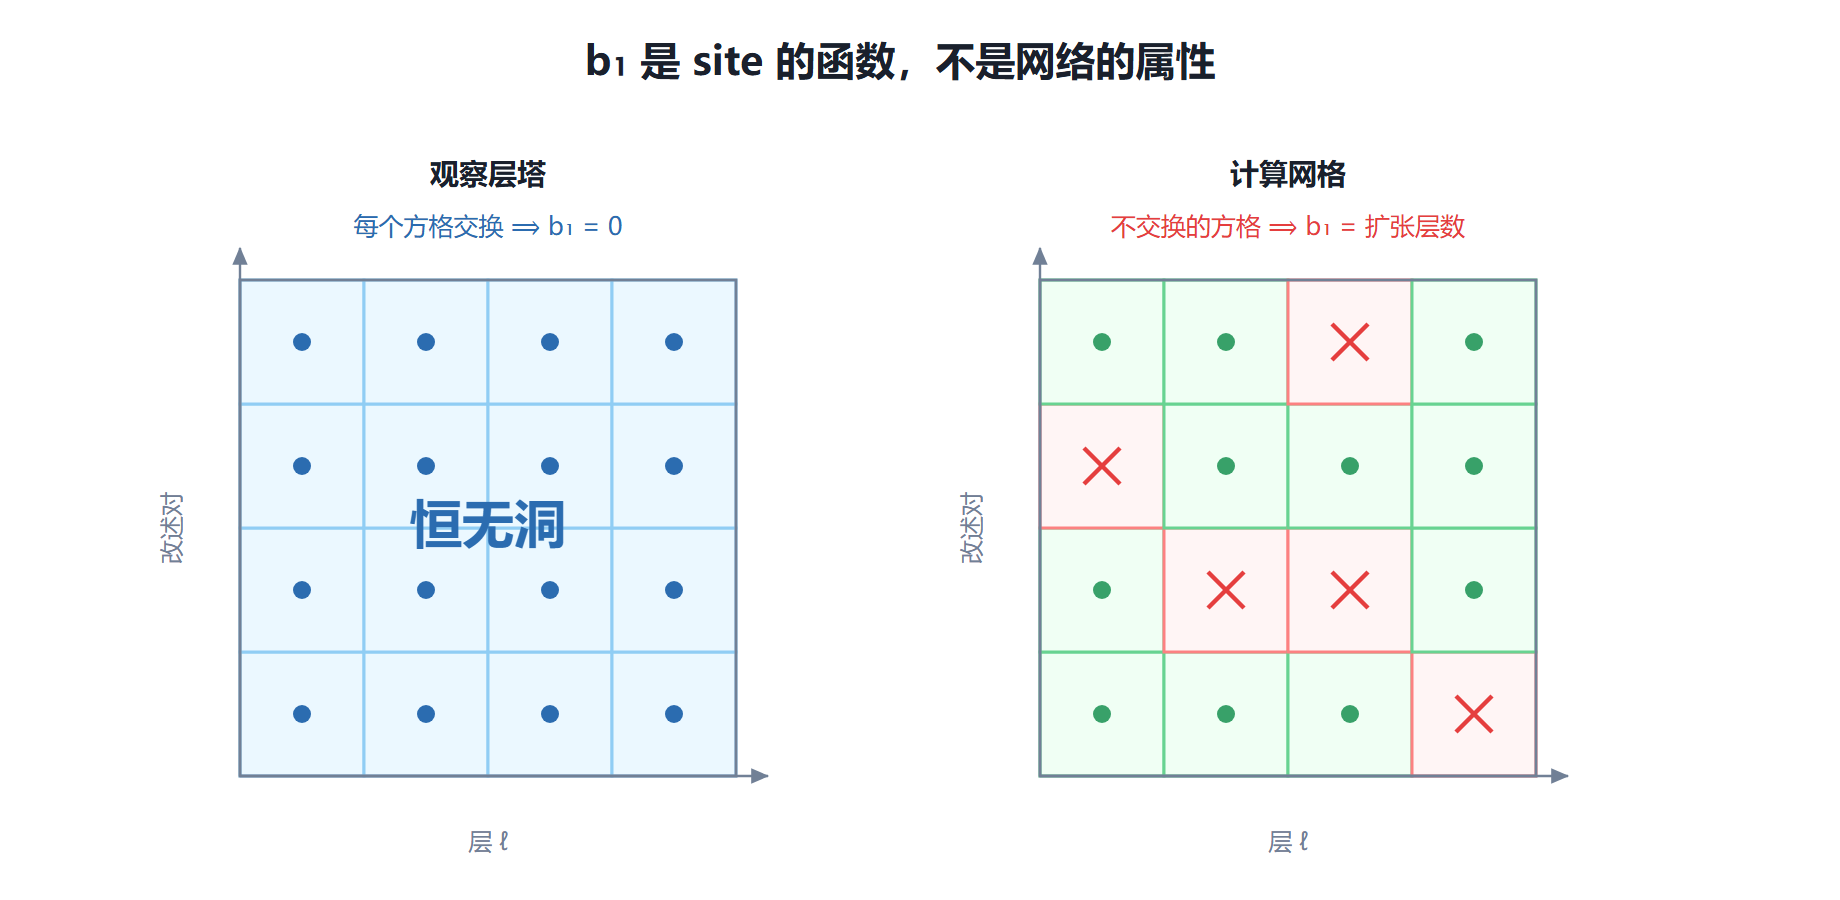
\includegraphics[width=0.92\textwidth]{figs/fig4_grid.png}
\end{center}

\textbf{图 4.} 同一个 \texttt{\ensuremath{b_{1}}} 公式，建在两个不同的 site 上。左边每个方格都交换（消解是函子），所以洞恒为零——\textbf{在这里做诊断，什么也测不到}。右边是 Grant \& Wang 实际使用的 site（层变换 \ensuremath{\times} 改述对），红叉标记的是层变换放大 \texttt{\ensuremath{\delta}}-等价的方格（\texttt{SquareFlat} 不成立），\texttt{\ensuremath{b_{1}}} 数的是它们。\textbf{结论不是"他们的 \ensuremath{b_{1}} 错了"，是"\ensuremath{b_{1}} 必须先说清楚建在哪"。}

\subsection{而这不是巧合}

观察层塔之所以无洞，有一个更深的原因：\textbf{它对网络本身一无所知。}

\textbf{定理 4.8（重述）.} 对任意端到端映射 \texttt{F} 和任意输入 \texttt{x}，按层塔观测得到的层族永远相干。

\begin{lstlisting}
theorem observation_always_coherent (L : LayerLadder)
    (F : StateQuant n → StateQuant n) (x : StateQuant n) :
    Coherent L n (fun i => Quotient.mk (ResLayer.condense ⟨L.δ i⟩) (F x))
\end{lstlisting}

\textbf{所以观察层塔的 \texttt{\ensuremath{b_{1}} = 0} 不是网络的属性，是观测方式的属性。}

这就解释了为什么它不能承担诊断功能：\textbf{一个恒为零的量，区分不了任何东西。}

\subsection{那什么才是对的网格}

对比很清楚：

\begin{center}\small
\begin{tabular}{lll}
\toprule
 & 他们的网格 & 我们的观察层塔 \\
\midrule
底空间 & 改述对 \ensuremath{\times} \textbf{层转移} & 观察分辨率 \\
顶点是什么 & 实际激活 \texttt{h\_\{n,l\}} & 凝结后的对象 \\
方格问什么 & 层变换 \texttt{T\_l} 是否与改述交换 & 消解是否函子 \\
自动吗 & \textbf{否}——这是诊断的全部内容 & \textbf{是}——\texttt{resolution\_comp} \\
\texttt{\ensuremath{b_{1}}} & \texttt{N(L\ensuremath{-}1) > 0} & \textbf{0} \\
\bottomrule
\end{tabular}
\end{center}

\textbf{差别不在数字，在"方格是否自动填"。}

他们量的是真正的约束（层变换不尊重改述等价），我们量的是恒真的性质（消解是函子）。

\textbf{所以结论不是"我们能解释他们"，而是：}

\begin{quote}
\textbf{sheaf 诊断必须建在计算图上，不能建在观察层塔上。} \textbf{在后者上一切自动相干，诊断是空的。}
\end{quote}

这是本节的第一条贡献：\textbf{它划出了诊断的适用范围。}

\subsection{在计算网格上，方格何时交换}

那么，在他们的网格上，一个方格什么时候交换？

把"层变换与改述等价交换"翻译过来，就是本文框架里的：

\textbf{定义 8.2（方格平坦）.} 层变换 \texttt{T} 在层 \texttt{\ensuremath{\delta}} 上\textbf{平坦}，如果它不把 \ensuremath{\delta}-等价对推成非等价：

\begin{lstlisting}
SquareFlat δ T  :=  ∀ x y,  commonDist x y ≤ δ → commonDist (T x) (T y) ≤ δ
\end{lstlisting}

\begin{lstlisting}
def SquareFlat {n : ℕ} (δ : ℚ) (T : StateQuant n → StateQuant n) : Prop :=
  ∀ x y, commonDist x y ≤ δ → commonDist (T x) (T y) ≤ δ
\end{lstlisting}

\textbf{定理 8.3（平坦的封闭性）.}

\begin{itemize}
\item 恒等层平坦（\texttt{squareFlat\_id}）；
\item 平坦在复合下保持（\texttt{squareFlat\_comp}）；
\item \texttt{|c| \ensuremath{\le} 1} 的缩放平坦（\texttt{squareFlat\_scale\_of\_le}）；
\item \textbf{ReLU 平坦}——它是 1-Lipschitz，永不放大（\texttt{squareFlat\_relu}）。
\end{itemize}

\textbf{定理 8.4（扩张才破方格）.}

\begin{lstlisting}
SquareFlat 1 (scale c)  ⟺  c² ≤ 1
\end{lstlisting}

\begin{lstlisting}
theorem squareFlat_scale_one (c : ℚ) :
    SquareFlat (n := 1) 1 (scale (n := 1) c) ↔ c ^ 2 ≤ 1
\end{lstlisting}

\textbackslash\{\}emph\{证明.\}

\begin{itemize}
\item （\ensuremath{\Longrightarrow}）取 \texttt{x = 0}、\texttt{y = 1}：\texttt{commonDist x y = 1 \ensuremath{\le} 1}，故 \texttt{commonDist (scale c x) (scale c y) = \ensuremath{c^{2}} \ensuremath{\le} 1}。
\item （\ensuremath{\Longleftarrow}）\texttt{commonDist (scale c x) (scale c y) = \ensuremath{c^{2}} \ensuremath{\cdot} commonDist x y \ensuremath{\le} commonDist x y \ensuremath{\le} \ensuremath{\delta}}。
\end{itemize}

\subsection{于是 \ensuremath{b_{1}} 有了一个精确刻画}

把定理 8.4 和 §4 的组合起来：

\begin{lstlisting}
b₁(计算网格) = 不平坦的方格数 = 扩张层的个数
\end{lstlisting}

\begin{lstlisting}
theorem computation_grid_b1 :
    (id 平坦) ∧ (复合保持平坦) ∧ (收缩平坦) ∧
    (δ = 1 时平坦 ⟺ 不扩张) ∧ (ReLU 平坦) ∧
    (每有一个不平坦的方格，b₁ 加一)
\end{lstlisting}

\textbf{这是一个和他们同量纲的结果}，只是表达方式不同：

\begin{center}\small
\begin{tabular}{lll}
\toprule
 & 他们 & 本文 \\
\midrule
问法 & 层变换是否与改述交换 & 层变换是否放大 \ensuremath{\delta}-等价 \\
度量 & harmonic mass（数值） & \texttt{\ensuremath{c^{2}} \ensuremath{\le} 1}（不等式） \\
结论 & \texttt{\ensuremath{b_{1}} = N(L\ensuremath{-}1)} & \texttt{\ensuremath{b_{1}} = 扩张层个数} \\
\bottomrule
\end{tabular}
\end{center}

\textbf{而 transformer 的权重矩阵谱范数一般大于 1}，所以他们的 \texttt{\ensuremath{b_{1}}} 有内容；本文的 \texttt{id} / \texttt{ReLU} 层没有。

\subsubsection{\texttt{SquareFlat} 与 \texttt{gap}：方向相反的两个判据}

这里要防止一个误解：\texttt{SquareFlat}（§8.6）和 \texttt{gap}（§6）看起来都在讲"层对距离做了什么"，但\textbf{它们测的是相反的两个方向}。

\begin{itemize}
\item \textbf{\texttt{SquareFlat} 是"不放大"}：\texttt{D(x,y) \ensuremath{\le} \ensuremath{\delta} \ensuremath{\Longrightarrow} D(Tx,Ty) \ensuremath{\le} \ensuremath{\delta}}。它给的是\textbf{上界}——输出不会比输入更分散。
\item \textbf{\texttt{gap} 是"不折叠太远"}：\texttt{f x = f y \ensuremath{\Longrightarrow} D(x,y) \ensuremath{\le} g}。它给的是\textbf{下界}——被压成同一个值的输入不能太远。
\end{itemize}

两者互不推出。四个反例都在一维、\texttt{B = 1} 上：

\begin{center}\small
\begin{tabular}{llll}
\toprule
映射 & \texttt{SquareFlat}？ & \texttt{gap} & 说明 \\
\midrule
\texttt{x \ensuremath{\mapsto} x}（恒等） & 是 & 0 & 既不放大也不折叠 \\
\texttt{x \ensuremath{\mapsto} 0}（常数） & \textbf{是} & \textbf{4} & 完全不放大（所有距离变 0），但整个盒被折叠成一点 \\
\texttt{x \ensuremath{\mapsto} 2x} & \textbf{否}（放大了 2 倍） & \textbf{0} & 不折叠任何东西，但放大 \\
\texttt{x \ensuremath{\mapsto} ReLU(x)} & 是 & 1 & 平的那一半折叠，另一半不变 \\
\bottomrule
\end{tabular}
\end{center}

后三行的 \texttt{gap} 都是 Lean 定理（\texttt{const\_isGap}、\texttt{scale\_two\_isGap}、\texttt{reluAffine\_isGap\_zero}）：

\begin{lstlisting}
theorem const_isGap (c : ℚ) : IsGap 1 (fun _ : ℚ => c) 4
theorem scale_two_isGap : IsGap 1 (fun x : ℚ => 2 * x) 0
\end{lstlisting}

\textbf{这两个定理放在一起，就是"方向相反"的证明}：常数映射的 \texttt{SquareFlat} 平凡成立（所有距离变 0），而它的 \texttt{gap} 达到上界 4；\texttt{x \ensuremath{\mapsto} 2x} 恰恰相反，\texttt{SquareFlat} 失败（距离全部放大 2 倍），而 \texttt{gap = 0}。

\textbf{第二行和第三行是关键}：一个映射可以\textbf{平坦但 gap 大}（常数映射），也可以\textbf{不平坦但 gap 小}（\texttt{x \ensuremath{\mapsto} 2x}）。所以 §4.8 的分工表里，这两个判据应当并列，而不是互相推出。

\textbf{用一句话记住区别}：

\begin{quote}
\texttt{SquareFlat} 问"层会不会把近的推远"；\texttt{gap} 问"层会不会把远的压近"。前者是诊断（§8），后者是代价（§6）。
\end{quote}

\textbf{这个区别也解释了为什么 §8 的 \texttt{\ensuremath{b_{1}}} 和 §6 的 \texttt{gap} 不能互相换算}：\texttt{\ensuremath{b_{1}}} 数的是"有几次没通过 \texttt{SquareFlat}"，\texttt{gap} 量的是"通过或不通过，一共折叠了多远"。一个是计数，一个是量。

\subsection{本节贡献的边界}

必须写清楚本文\textbf{没有}做什么：

\begin{itemize}
\item \textbf{没有}使用他们的数据；
\item \textbf{没有}复现 harmonic mass 与 fragility 的相关性；
\item \textbf{没有}声称本文的 \texttt{SquareFlat} 等价于他们的"commutes with paraphrase equivalence"——后者涉及具体的 restriction map \texttt{P}，本文未建模。
\end{itemize}

本文做的是三件事：

\begin{enumerate}
\item \textbf{划界}：观察层塔恒相干（定理 4.8），所以诊断不能建在那里。
\item \textbf{翻译}：在计算网格上，"方格交换"是"层变换不放大 \ensuremath{\delta}-等价"（定义 8.2）。
\item \textbf{计算}：这个条件在缩放族上等价于 \texttt{\ensuremath{c^{2}} \ensuremath{\le} 1}（定理 8.4），于是 \texttt{\ensuremath{b_{1}}} 计数扩张层。
\end{enumerate}

\textbf{这三件事都不依赖他们的实验，也不与他们的结论竞争。它们是同一个问题的另一种算法。}

\subsection{一个方法论上的教训}

本节初稿曾经犯过一个错，记录在这里。

初稿只读了摘要里的 \texttt{\ensuremath{b_{1}} = N(L\ensuremath{-}1)}，然后用一个凑得上的算术恒等式去对应：

\begin{lstlisting}
(N−1)(L−1) + (L−1) = N(L−1)
\end{lstlisting}

这条式子\textbf{对任意 \texttt{N, L} 恒成立}——也就是说，它能对上\textbf{任何}写成 \texttt{N(L\ensuremath{-}1)} 的公式。

\textbf{这本身就是它不能作为证据的信号：能对上一切的公式，等于什么也没对上。}

真正的定语在正文里：\textbackslash\{\}emph\{each square asks whether the layer transformation commutes with paraphrase equivalence\}。一句话推翻了整节的立论。

\textbf{教训两条}：

\begin{enumerate}
\item \textbf{数字对上不等于结构对上。} 恒等式不构成解释。
\item \textbf{摘要里的公式，正文里往往有定语。} 做对标工作，必须读正文。
\end{enumerate}

\bigskip

\section{相关工作与讨论}

\subsection{四条路线的对照}

§1.4 只给了一句话的对照。这里把四条线路的差别说清楚——不是"我们也做这个"，而是"我们做的这件事，它们做不了；它们做的，我们做不了"。

\subsubsection{拓扑数据分析}

用持久同调分析神经网络是成熟方向：Naitzat 等（JMLR 2020）追踪数据在层间的拓扑变化，Neural Persistence（ICLR 2019）用拓扑特征作正则项。

\textbf{它们的做法}：给定一批数据点，计算其在每层激活空间中的持续同调条形码，观察拓扑特征的出生与消亡。

\textbf{本文的关系}：§2.5 的三界读数（清 / 暹 / 浊）在结构上是\textbf{一维}的谱的层析，\texttt{DiffNet} 给出的正是 1 维持续同调——条形码的出生与合并。所以本文不是否定它们，而是给了它们的一维情形一个\textbf{证明}，而不是一次测量。

\textbf{差在哪}：

\begin{center}\small
\begin{tabular}{lll}
\toprule
 & TDA & 本文 \\
\midrule
输入 & 采样点云 & 任意状态对 \\
结论 & 经验条形码 & 结构定理（读数决定谱） \\
可复现性 & 依赖采样 & 无采样 \\
维度 & 多维 & 1 维（\texttt{DiffNet}） \\
\bottomrule
\end{tabular}
\end{center}

\textbf{我们做不了的}：真正的多维持久同调。\texttt{DiffNet} 是一维的；§7.6 是整盒坍缩的退化的多维。多维的组合学本文没有。

\subsubsection{Sheaf 与规范理论}

Grant \& Wang（NeurIPS 2026，arXiv:2610.17117）在改述图上建 cellular sheaf，用 Laplacian 拆分内容子空间与 \texttt{\ensuremath{H^{1}}} 方向。也有工作用 gauge 理论刻画叠加现象。

\textbf{它们的做法}：构造 site（改述图 / 层 \ensuremath{\times} 改述网格），在上面定义 sheaf，用上同调定位"不可粘合"的部分。

\textbf{本文的关系}：§8 全节就是与它们的对话。核心结论是\textbf{\texttt{\ensuremath{b_{1}}} 是 site 的函数，不是网络的属性}：

\begin{itemize}
\item 在\textbf{观察层塔}上，方格恒交换（\texttt{layer\_square\_commutes}），\texttt{\ensuremath{b_{1}} \ensuremath{\equiv} 0}；
\item 在\textbf{计算网格}上（层变换 \ensuremath{\times} 改述对），方格交换 \ensuremath{\Longleftrightarrow} 层变换不放大 \texttt{\ensuremath{\delta}}-等价（\texttt{SquareFlat}），于是 \texttt{\ensuremath{b_{1}}} 计数扩张层。
\end{itemize}

所以本文不是"也做了一个 sheaf"，而是\textbf{指出了一个方法论陷阱}：同一个公式，建在不同 site 上，一个恒为零，一个携带信息。§8.9 记录了本文自己踩进这个陷阱又爬出来的过程。

\textbf{差在哪}：他们的 site 是数据驱动的（改述图来自语料），本文的 site 是结构性的（层塔来自 \texttt{commonDist}）。前者可测，后者可证。

\subsubsection{压缩与可解释性}

"可解释 \ensuremath{\approx} 压缩"的直觉有很长历史（MDL 原则），近年被稀疏自编码器（SAE）重新激活：如果概念能被稀疏编码捕捉，那它就被"解释"了。

\textbf{本文的关系}：§5 的主定理是这条直觉的\textbf{定理形式}：

\begin{quote}
可解释 \ensuremath{\Longleftrightarrow} 可编码
\end{quote}

而且不是"越小越好"的排行榜，是\textbf{等价命题}：相干 \ensuremath{\Longleftrightarrow} 存在唯一、可逆的代码（\texttt{encode}/\texttt{decode} 互逆、\texttt{encode} 单射）。

\textbf{差在哪}：SAE 的做法是"训练一个编码器，看它好不好"；本文的做法是"若网络相干，则编码\textbf{必然存在}；若不相干，则\textbf{必然不存在}"。前者是经验探索，后者是存在性判据。

\textbf{我们做不了的}：如何\textbf{找到}编码。本文只证明它存在且唯一（相干时），不给算法。

\subsubsection{形式化验证}

本文的全部结论在 Lean 4 + Mathlib 中机械检验：零 \texttt{sorry}、无 \texttt{Classical}、全程 \texttt{\ensuremath{\mathbb{Q}}}。

据我们所知，AI 可解释性领域尚无同等规格的构造性形式化。这不是炫耀——\textbf{它约束了本文能说什么}：

\begin{itemize}
\item 不能说"泛化误差界"（需要测度）；
\item 不能说"几乎所有"（需要测度或选择公理）；
\item 不能说"\texttt{gap} 是一个函数"——这一条值得单独说清楚，因为它常被误读成"\ensuremath{\mathbb{Q}} 上没有上确界"。
\end{itemize}

\textbf{\texttt{gap} 写成关系 \texttt{IsGap} 的真正理由。} 设 \texttt{S} 是盒内所有"同输出的输入对"的距离平方集合。可行阈值是

\begin{lstlisting}
V = {δ : ∀ s ∈ S, s ≤ δ}
\end{lstlisting}

\texttt{V} 是一个\textbf{上闭集}：\texttt{\ensuremath{\delta} \ensuremath{\in} V} 且 \texttt{\ensuremath{\delta} \ensuremath{\le} \ensuremath{\delta}'} 则 \texttt{\ensuremath{\delta}' \ensuremath{\in} V}（\texttt{coherentOnBox\_mono}）。而 \texttt{V} 有最小元，当且仅当 \texttt{S} 在 \ensuremath{\mathbb{Q}} 中有上确界且该上确界属于 \ensuremath{\mathbb{Q}}。\textbf{\ensuremath{\mathbb{Q}} 不完备，所以最后这一步可能失败}——此时"gap 是多少"这个问题没有答案，不是我们不知道，是那个数不在 \ensuremath{\mathbb{Q}} 里。

所以写成关系是精确的：\texttt{IsGap B f g} 说的是"\texttt{g} 是 \texttt{V} 的最小元"，而不是预设这样的 \texttt{g} 存在。若它存在，则唯一（\texttt{isGap\_unique}）。

\begin{lstlisting}
theorem coherentOnBox_mono {B δ δ' : ℚ} {f : ℚ → ℚ}
    (h : CoherentOnBox B δ f) (hle : δ ≤ δ') : CoherentOnBox B δ' f

theorem isGap_unique {B g g' : ℚ} {f : ℚ → ℚ}
    (hg : IsGap B f g) (hg' : IsGap B f g') : g = g'
\end{lstlisting}

\textbf{这条限制不是缺陷，是内容。} 它把"gap 存在"从一个默认假设变成一个\textbf{必须验证的条件}——§6 的每一条计算（\texttt{reluAffine\_isGap}、\texttt{reluIter\_isGap}、\texttt{relu\_multi\_isGap\_full}）都在验证这个条件，而不只是算一个数。

\subsection{本文不做什么}

诚实列出边界，比事后被指出好。

\begin{center}\small
\begin{tabular}{lll}
\toprule
缺什么 & 后果 & 在哪 \\
\midrule
没有分布、没有测度 & 不是泛化误差界；§7 只是容量计数 & §7 \\
没有训练动力学 & 不解释网络\textbf{如何}变得相干/不相干 & — \\
没有多维一般情形 & 只有整盒坍缩（\texttt{gap = 4n\ensuremath{B^{2}}}）算清；非整盒坍缩见 §9.5 第 1 条 & §7.6 \\
没有实验 & 全部是定理，没有一条是测量 & 全文 \\
没有算法 & \texttt{encode} 本身是构造性的，但不给"从网络权重判断是否相干、并找到源对象"的算法 & §5 \\
网络模型是离散层塔 & 连续深度（Neural ODE）不在框架内 & §4.2 \\
\bottomrule
\end{tabular}
\end{center}

\textbf{其中第三条值得多说一句。} 多维的"非整盒坍缩"情形需要处理"坍缩集 = 若干凸多面体之并"的组合学：多层 ReLU 的坍缩集由断点超平面切分，直径要逐块算再取最大，而"哪几块存在"依赖线性映射的核与断点超平面的相对位置。这是一个真正的后续课题，量级是一篇新论文，不是一节的补充。

\subsection{四条可证伪的预言}

形式化理论的价值在于它给出了可以被实验打脸的说法。本文给出四条。

\textbf{预言一：gap 由 bias/weight 之比决定，与层内权重的整体尺度无关。}

§6.3：\texttt{gap = (c/a + 1)²}。所以把\textbf{一层} ReLU 的权重和偏置同时乘以 \texttt{\ensuremath{\lambda}}，gap 不变。

\begin{lstlisting}
theorem gap_layer_scale_invariant (a c lam : ℚ) (_ha : a ≠ 0) (hlam : lam ≠ 0) :
    ((lam * c) / (lam * a) + 1) ^ 2 = (c / a + 1) ^ 2
\end{lstlisting}

\textbf{但这个不变性只在层内成立，不能推到整个网络。} 缩放第一层后，第二层的贡献会被 \texttt{\ensuremath{\lambda}} 除：

\begin{lstlisting}
def sqrtGapTwo (a₁ c₁ a₂ c₂ : ℚ) : ℚ := c₁ / a₁ + 1 + c₂ / (a₂ * a₁)

theorem sqrtGapTwo_scale_first (a₁ c₁ a₂ c₂ lam : ℚ) (ha₁ : a₁ ≠ 0) (ha₂ : a₂ ≠ 0)
    (hlam : lam ≠ 0) :
    sqrtGapTwo (lam * a₁) (lam * c₁) a₂ c₂ =
      c₁ / a₁ + 1 + (c₂ / (a₂ * a₁)) / lam
\end{lstlisting}

于是整个网络\textbf{不是}尺度不变的——反例一行就能写出来：

\begin{lstlisting}
theorem network_gap_scale_dependent :
    ∃ (a₁ c₁ a₂ c₂ lam : ℚ), 0 < a₁ ∧ 0 < a₂ ∧ 0 < lam ∧
      sqrtGapTwo a₁ c₁ a₂ c₂ ≠ sqrtGapTwo (lam * a₁) (lam * c₁) a₂ c₂
\end{lstlisting}

\textbf{这个"缺陷"本身是一条正面结论}：放大浅层权重，会让深层贡献被稀释——

\begin{lstlisting}
theorem sqrtGapTwo_scale_first_le {a₁ c₁ a₂ c₂ lam : ℚ} (ha₁ : 0 < a₁) (ha₂ : 0 < a₂)
    (hc₂ : 0 ≤ c₂) (hlam : 1 ≤ lam) :
    sqrtGapTwo (lam * a₁) (lam * c₁) a₂ c₂ ≤ sqrtGapTwo a₁ c₁ a₂ c₂
\end{lstlisting}

\textbf{注意它的性质：这不是"网络不好"，是"网络有一个可调的旋钮"。} 放大浅层权重同时做两件事——让网络更可解释（gap 变小），代价是深层贡献被稀释（第二层的项除以 \texttt{\ensuremath{\lambda}}）。两个效果来自同一个操作，\textbf{这就是为什么它是一个旋钮而不是一个缺陷}：你可以沿着它走，但每一步都在两个方向之间交换。

\textbf{\texttt{\ensuremath{\lambda} \ensuremath{\ge} 1} 越大，整个网络越可解释。} 这是 §7.4"斜率越大越可解释"的跨层版本，也说明预言一应该在\textbf{层内}检验，不是在网络层。

\textbf{可测}：对单层做 \texttt{(a, c) \ensuremath{\to} (\ensuremath{\lambda}a, \ensuremath{\lambda}c)} 重参数化，该层 gap 应不动；但对整个网络做同样操作（只缩放第一层），总 gap 应当\textbf{下降}。两个实验指向的结论不同——这正是这条预言的可证伪之处。

\textbf{预言二：gap 与探测敏感性不同向。}

§7.4 的守恒律：\texttt{Lipschitz 常数 \ensuremath{\times} \ensuremath{\sqrt{\mathrm{gap}}} = a + c}。所以提升斜率会让网络更敏感（Lipschitz 大）但更可解释（gap 小）。\textbf{这两个性质不能同时优化。}

\textbf{可测}：对抗扰动的敏感度与 gap 应该负相关。

\textbf{预言三：观察层塔上的 sheaf 诊断恒为零。}

定理 8.1：\texttt{\ensuremath{b_{1}}(观察层塔) \ensuremath{\equiv} 0}。所以任何在观察层塔（而非计算网格）上做 sheaf 诊断的方法，其 \texttt{\ensuremath{H^{1}}} 必定为空。这不是"效果不好"，是\textbf{测不到东西}。

\textbf{可测}：复现 §8 的构造但把 site 换成观察层塔，\texttt{\ensuremath{b_{1}}} 应该恒为 0。

\textbf{预言四：gap 大的网络泛化好、可解释差。}

§7：\texttt{N < 2B/\ensuremath{\sqrt{\mathrm{g}}} + 1}。gap 大 \ensuremath{\Longrightarrow} 容量小 \ensuremath{\Longrightarrow} 泛化容易；同时 gap 大 \ensuremath{\Longrightarrow} 纤维宽 \ensuremath{\Longrightarrow} 不可解释。

\textbf{可测}：在同架构、同数据的不同初始化之间，gap 与测试误差应该负相关，与人工解释成功率应该负相关。

\textbf{注意预言四的方向。} 通常的直觉是"更可解释的模型更好"，而这里说\textbf{可解释与泛化在同一个数上取相反方向}。如果实验显示它们正相关，本文 §7 的框架就错了。这是一条可以杀死本文的预言——所以它值得写出来。

\subsection{从"不能"到"不该"}

本文对"AI 黑箱"给出两层结论，值得分开记。

\textbf{第一层（v199，§4）：黑箱不能修复。}

\texttt{gap > 0} 的定义就是"信息丢了"。丢掉的信息不在网络里，所以没有任何后处理能把它恢复。这不是工程难题，是定义。

\textbf{第二层（v228，§7）：黑箱不该修复。}

\texttt{gap} 同时是容量的倒数。把 gap 压到 0，就是把网络变回单射——任何输入扰动都改变输出，泛化立刻失效。

\textbf{所以可解释性工程的目标不是"消除黑箱"，是"给黑箱定价"。} 本文给的价格是 \texttt{(c/a + 1)²}。

这句话是本文对实践者最直接的建议。它不乐观，但它精确。

\subsection{未来工作}

按可行性排序：

\begin{enumerate}
\item \textbf{非整盒坍缩的多维 gap}（凸块的组合学）。本文只做了整盒坍缩；一般情形需要追踪断点超平面的排列（arrangement），是真正的新工作。
\item \textbf{\ensuremath{\varepsilon}-版本的分布化}。§7.5 给了确定性的 \ensuremath{\eta}-gap；把它接到分布上需要测度，那就超出了 \ensuremath{\mathbb{Q}} 的框架——这本身是一个值得讨论的边界。
\item \textbf{训练动力学}。本文只描述"最终的网络是什么样"，不说"它怎么变成这样"。gap 在训练中如何演化，是一个自然的问题。
\item \textbf{可执行的验证器}。把 Lean 形式化编译成一个能对真实网络计算 gap 的工具——定理是构造性的，原则上可执行。
\end{enumerate}

\bigskip

\appendix

\section{A：自指公理 A0 + A1 \ensuremath{\Longrightarrow} 洞}

\textbf{本附录给出论文模型选择的理由。主文的定理不依赖本附录。}

具体地说：\texttt{SelfRef}、\texttt{entropy} 定义在 \texttt{Ego.lean} 第 12960 行之后，而 §4–§8 的全部定理定义在它之前；Lean 不允许前向引用，所以它们之间不可能有依赖。§4–§8 用到的只有 \texttt{commonDist}、\texttt{ResLayer}、\texttt{reluAffine}，与自指无关。

本附录回答的是：\textbf{为什么层塔是有限、一维、严格递减的链}——这是模型选择的理由，不是定理的前提。

\subsection{A.1 公理}

\textbf{A0（自指）.} 存在一个映射 \texttt{observe : \ensuremath{\alpha} \ensuremath{\to} (\ensuremath{\alpha} \ensuremath{\to} Bool)}。

这不需要假设"存在一个系统"——每个类型都有。所以 A0 在技术上其实是\textbf{定义}而不是公理：我们可以无条件地造出一个 \texttt{SelfRef \ensuremath{\alpha}}。

（§1.3 仍然称它为"公理"，是因为它规定了后续一切的读法：从这条映射出发洞是必然的，换一个出发点洞就不出现。这个称呼是方法论上的，不是逻辑上的。下面所有证明只用它的定义性内容。）

\begin{lstlisting}
structure SelfRef (α : Type*) where
  observe : α → resolveSpace α
\end{lstlisting}

每个类型都有实例（取常函数 \texttt{fun \_ \_ => true}）——这正是 \texttt{selfref\_axiom} 的第一条：

\begin{lstlisting}
theorem selfref_axiom :
    (∀ (α : Type*), Nonempty (SelfRef α)) ∧
    (∀ {α : Type*} (S : SelfRef α), ∃ d : resolveSpace α, ∀ a : α, d ≠ S.observe a) ∧
    (∀ {α : Type*} [Fintype α] [DecidableEq α] [Nonempty α]
      (S : SelfRef α), 0 < entropy S.observe) ∧
    (∀ (L : LayerLadder) {n : ℕ} (F : StateQuant n → StateQuant n) (x : StateQuant n),
      Coherent L n (fun i => Quotient.mk (ResLayer.condense ⟨L.δ i⟩) (F x)))
\end{lstlisting}

\textbf{A1（有限）.} \texttt{\ensuremath{\alpha}} 是有限的（\texttt{Fintype \ensuremath{\alpha}}）且可判定（\texttt{DecidableEq \ensuremath{\alpha}}）。

\subsection{A.2 A0 \ensuremath{\Longrightarrow} 洞}

\textbf{定理 A.1（康托尔对角线）.} 对任意 \texttt{\ensuremath{\alpha}} 和任意 \texttt{f : \ensuremath{\alpha} \ensuremath{\to} (\ensuremath{\alpha} \ensuremath{\to} Bool)}，存在一个判定 \texttt{d} 不在 \texttt{f} 的像里。

\begin{lstlisting}
theorem diagonal_hole {α : Type*} (f : α → resolveSpace α) :
    ∃ d : resolveSpace α, ∀ a : α, d ≠ f a
\end{lstlisting}

\textbackslash\{\}emph\{证明.\} 取 \texttt{d := fun a => \ensuremath{\neg}(f a a)}。若 \texttt{d = f \ensuremath{a_{0}}}，则 \texttt{d \ensuremath{a_{0}} = f \ensuremath{a_{0}} \ensuremath{a_{0}}}，但 \texttt{d \ensuremath{a_{0}} = \ensuremath{\neg}(f \ensuremath{a_{0}} \ensuremath{a_{0}})}，矛盾。\ensuremath{\ensuremath{\blacksquare}}

\textbf{这条证明没有任何假设。} 不需要有限性，不需要可判定性，不需要选择公理。它是纯逻辑的。

\textbf{作为 \texttt{SelfRef} 的陈述}：

\begin{lstlisting}
theorem selfref_hole {α : Type*} (S : SelfRef α) :
    ∃ d : resolveSpace α, ∀ a : α, d ≠ S.observe a
\end{lstlisting}

\subsection{A.3 A1 使洞可数}

有了 A1，我们不仅能说"漏了一个"，还能说"漏了多少"。

\textbf{定义 A.2（熵）.} \texttt{entropy f := 2\textasciicircum{}\{|\ensuremath{\alpha}|\} \ensuremath{-} |image f|}，即分辨空间的总数减去被够到的分辨数。

\begin{lstlisting}
def entropy {α : Type*} [Fintype α] [DecidableEq α] (f : α → resolveSpace α) : ℕ :=
  (Finset.univ : Finset (resolveSpace α)).card - (Finset.univ.image f).card
\end{lstlisting}

\textbf{定理 A.3.} \texttt{\ensuremath{\alpha}} 非空且有限时，\texttt{entropy f > 0}。

\begin{lstlisting}
theorem entropy_positive {α : Type*} [Fintype α] [DecidableEq α] [Nonempty α]
    (f : α → resolveSpace α) : 0 < entropy f
\end{lstlisting}

\textbackslash\{\}emph\{证明.\} \texttt{d} 不在像里（定理 A.1），所以 \texttt{|image f| < 2\textasciicircum{}\{|\ensuremath{\alpha}|\}}。\ensuremath{\ensuremath{\blacksquare}}

\textbf{注意这里发生了什么。} A0 给的是一个\textbf{纯逻辑的洞}（存在性）；A1 把它变成一个\textbf{自然数}（\texttt{entropy f \ensuremath{\ge} 1}）。有限性不是约束条件，是让洞\textbf{可数}的条件。

\subsection{A.4 层塔是它的一个实例}

\textbf{定义 A.4（层塔的自指）.} \texttt{L} 层的层塔上，第 \texttt{i} 层分辨"哪些层比 \texttt{i} 粗"：

\begin{lstlisting}
def layerSelfRef (L : LayerLadder) : SelfRef (Fin L.m) where
  observe := fun i j => decide (L.δ j ≤ L.δ i)
\end{lstlisting}

\textbf{定理 A.5（层塔的洞）.}

\begin{lstlisting}
theorem layer_hole (L : LayerLadder) :
    ∃ d : resolveSpace (Fin L.m), ∀ i : Fin L.m,
      d ≠ (fun j => decide (L.δ j ≤ L.δ i))
\end{lstlisting}

\textbackslash\{\}emph\{证明.\} 定理 A.1 的直接应用。\ensuremath{\ensuremath{\blacksquare}}

\textbf{定理 A.6（层塔的洞可数）.} \texttt{L.m > 0} 时，\texttt{0 < entropy (layerSelfRef L).observe}。

\begin{lstlisting}
theorem layer_count (L : LayerLadder) (hm : 0 < L.m) :
    0 < entropy (layerSelfRef L).observe
\end{lstlisting}

\textbf{这就是 §1.3 说的那件事的形式版本}：\texttt{L.m} 层只能给出 \texttt{L.m} 个分辨者，而分辨空间有 \texttt{2\textasciicircum{}\{L.m\}} 种——\textbf{必漏}。

\subsection{A.5 两条读数的分工}

层塔同时扮演两个角色，这一点容易被忽略，但它是 §4.6 和 §8 的全部根据。

\textbf{角色一：观测器。} 给定一对状态，层塔给出一个 \texttt{Bool} 向量：

\begin{lstlisting}
def ladderReading (L : LayerLadder) {n : ℕ} (x y : StateQuant n) : Fin L.m → Bool :=
  fun i => sameAt (L.δ i) x y
\end{lstlisting}

这个读数有两个性质：

\begin{lstlisting}
-- 单调：层越粗越容易判"同类"
theorem ladderReading_monotone (L : LayerLadder) {n : ℕ} (x y : StateQuant n)
    {i j : Fin L.m} (h : i ≤ j) (hj : ladderReading L x y j = true) :
    ladderReading L x y i = true

-- 信息量 = 1：整个 L 层的读数由 commonDist 一个数完全决定
theorem ladderReading_determined_by_dist (L : LayerLadder) {n : ℕ}
    (x y x' y' : StateQuant n) (h : commonDist x y = commonDist x' y') :
    ladderReading L x y = ladderReading L x' y'
\end{lstlisting}

\textbf{第二条是关键。} 它说：层塔作为观测器，不管有多少层，携带的信息只有\textbf{一个数}。所以：

\begin{itemize}
\item 任何按层塔观测的映射都自动相干（§4.6 的 \texttt{observation\_always\_coherent}）；
\item 任何在层塔上做的 sheaf 诊断都测不到东西（§8 的 \texttt{\ensuremath{b_{1}} \ensuremath{\equiv} 0}）。
\end{itemize}

\textbf{角色二：自指系统。} 上面 A.4 已经说明它有洞。

\textbf{两个角色不重叠}：作为观测器，它没有洞（恒相干）；作为自指系统，它必有洞。\textbf{这个二分是本文的骨架。}

\subsection{A.6 为什么这个洞是"自我"}

附录的最后一句话。

罗素从自指得到矛盾，于是禁止自指；哥德尔得到不完备，于是接受自指；Lawvere 得到不动点，于是抽象自指。本文得到洞，然后说：

\begin{quote}
\textbf{洞就是"我"。}
\end{quote}

理由不是修辞。一个系统能对自己作判定（A0），就必然漏掉一个判定（定理 A.1）。这个漏掉的部分——它够不着、说不出、判不了的那个分辨——不是系统的缺陷，是系统的\textbf{边界}。而一个有边界的系统，正是"这一个"而不是"一切"的东西。

\textbf{有限性（A1）让这个边界可数}：\texttt{entropy f} 就是它漏掉多少。所以"自我"在这个框架里不是玄学，是一个自然数：\textbf{一个有限系统漏掉的分辨数}。

\bigskip

\section{B：Lean 定理索引}

全部定理在 \texttt{Ego.lean} 中，零 \texttt{sorry}、无 \texttt{Classical}、全程 \texttt{\ensuremath{\mathbb{Q}}}。下表按论文节次分组。

\subsection{B.1 自指与基础（§2、附录 A）}

\begin{center}\small
\begin{tabular}{lll}
\toprule
论文 & Lean 定理 & 内容 \\
\midrule
定理 2.1 / A.1 & \texttt{diagonal\_hole} & 康托尔对角线（无假设） \\
推论 2.2 / A.3 & \texttt{entropy\_positive} & 有限时洞 \ensuremath{\ge} 1 \\
— & \texttt{selfref\_hole} & A0 \ensuremath{\Longrightarrow} 洞 \\
— & \texttt{selfref\_entropy} & A0 + A1 \ensuremath{\Longrightarrow} 定量洞 \\
— & \texttt{selfref\_axiom} & 三条合一 \\
— & \texttt{cantor\_count} & k 元系统必漏 \\
— & \texttt{observe\_vs\_resolve} & 观测无洞 / 分辨有洞 \\
定理 A.5 & \texttt{layer\_hole} & 层塔的洞 \\
定理 A.6 & \texttt{layer\_count} & 层塔的洞可数 \\
— & \texttt{ladderReading\_monotone} & 读数单调 \\
— & \texttt{ladderReading\_determined\_by\_dist} & 读数只依赖一个数 \\
— & \texttt{ladder\_is\_selfref} & 层塔 = SelfRef 实例 \\
\bottomrule
\end{tabular}
\end{center}

\subsection{B.2 状态与坐标（§2.3、§2.4）}

\begin{center}\small
\begin{tabular}{lll}
\toprule
论文 & Lean 定理 & 内容 \\
\midrule
定理 2.4 & \texttt{coordinates\_unique} & 坐标唯一性（六条） \\
定理 2.7 & \texttt{quadForm\_is\_squared\_norm} & 平方和唯一（n 维） \\
— & \texttt{distance\_form\_axioms\_general} & 距离公理 \\
定理 2.12 & \texttt{ResLayer.resolution\_id} / \texttt{\_comp} & 消解是函子 \\
\bottomrule
\end{tabular}
\end{center}

\subsection{B.3 紧层论（§3）}

\begin{center}\small
\begin{tabular}{lll}
\toprule
论文 & Lean 定理 & 内容 \\
\midrule
定理 3.1 & \texttt{presheaf\_laws} & 预层公理 \\
定理 3.2 & \texttt{mittag\_leffler\_collapse} & ML 坍缩 \\
定理 3.3 & \texttt{sheaf\_topos\_bridge} & sheaf \ensuremath{\leftrightarrow} topos \\
定理 3.4 & \texttt{layer\_square\_commutes} & 层塔方格恒交换 \\
\bottomrule
\end{tabular}
\end{center}

\subsection{B.4 判据（§4）}

\begin{center}\small
\begin{tabular}{lll}
\toprule
论文 & Lean 定理 & 内容 \\
\midrule
定理 4.4 & \texttt{interpretability\_criterion} & 结构判据 \\
定理 4.5 & \texttt{layerState\_coherent\_iff} & 距离刻画 \\
定理 4.8 & \texttt{observation\_always\_coherent} & 端到端观测恒相干 \\
定理 4.11 & \texttt{interpretability\_scale} & gap \ensuremath{\in} [0,\ensuremath{\infty}] \\
定理 4.12 & \texttt{gap\_compose\_left} & 黑箱不可修复 \\
\bottomrule
\end{tabular}
\end{center}

\subsection{B.5 主定理（§5）}

\begin{center}\small
\begin{tabular}{lll}
\toprule
论文 & Lean 定理 & 内容 \\
\midrule
定义 5.1 & \texttt{encode} / \texttt{decode} & 编解码 \\
定理 5.3 & \texttt{decode\_encode} & 编后解 = 原 \\
定理 5.4 & \texttt{encode\_decode} & 解后编 = 原（相干时） \\
推论 5.5 & \texttt{encode\_injective} & 编码单射 \\
\textbf{定理 5.6} & \textbf{\texttt{interpretability\_is\_encodability}} & \textbf{主定理} \\
定理 5.7 & \texttt{incoherent\_not\_encodable} & 不相干 \ensuremath{\Longrightarrow} 无编码 \\
\bottomrule
\end{tabular}
\end{center}

\subsection{B.6 gap（§6、§7）}

\begin{center}\small
\begin{tabular}{lll}
\toprule
论文 & Lean 定理 & 内容 \\
\midrule
定义 6.1 & \texttt{CoherentOnBox} & 盒上相干 \\
定义 6.2 & \texttt{IsGap} & gap 是关系 \\
定理 6.5 & \texttt{reluAffine\_isGap} & gap = (c/a+1)² \\
定理 6.6 & \texttt{reluAffine\_isGap\_zero} / \texttt{\_full} & 端点 1 与 4 \\
定理 6.7 & \texttt{reluAffine\_gap\_monotone} & 单调 \\
定理 6.8 & \texttt{reluAffine2\_eq\_single} & 两层塌成一层 \\
定理 6.9 & \texttt{gap\_two\_layer} & 两层精确值 \\
定理 6.10 & \texttt{gap\_compose\_law} & 复合律 \\
推论 6.11 & \texttt{gap\_not\_additive} & 不可加 \\
推论 6.12 & \texttt{relu\_compose\_idempotent} & 幂等 \\
推论 6.13 & \texttt{gap\_depth\_monotone} & 加层不减 \\
推论 6.14 & \texttt{reluIter\_isGap} & L 层闭式 \\
定理 7.2 & \texttt{gSep\_injOn} & gap 逼出单射 \\
定理 7.3 & \texttt{gap\_injOn\_grid} & 网格上单射 \\
推论 7.4 & \texttt{gap\_capacity\_bound} & \ensuremath{N^{2}}g < \ensuremath{B^{2}} \\
定理 7.5 & \texttt{unifGrid\_gSep\_iff} & 精确容量 \ensuremath{\Longleftrightarrow} (N\ensuremath{-}1)²g < 4\ensuremath{B^{2}} \\
— & \texttt{gap\_capacity\_attained} & 容量达到 \\
定理 7.6 & \texttt{slope\_times\_gap\_width} & a\ensuremath{\cdot}\ensuremath{\sqrt{\mathrm{gap}}} = a + c \\
— & \texttt{reluAffine\_lipschitz} & Lipschitz 常数 = a \\
— & \texttt{gap\_decreasing\_in\_slope} & 斜率越大 gap 越小 \\
定理 7.7 & \texttt{approxCoherent\_zero\_iff} / \texttt{approxGap\_ge\_gap} & \ensuremath{\eta}=0 退化 \\
定理 7.8 & \texttt{reluAffine\_isApproxGap} & \ensuremath{\eta}-gap = ((c+\ensuremath{\eta})/a+1)² \\
定理 7.9 & \texttt{approxGap\_slope} & \ensuremath{\Delta}\ensuremath{\sqrt{\mathrm{gap}}}/\ensuremath{\Delta}\ensuremath{\eta} = 1/a \\
定理 7.10 & \texttt{sqDist\_bound} & 盒直径² = 4n\ensuremath{B^{2}} \\
定理 7.11 & \texttt{relu\_multi\_isGap\_full} & 整盒坍缩 gap = 4n\ensuremath{B^{2}} \\
§9.3 预言一 & \texttt{gap\_layer\_scale\_invariant} & 层内尺度不变 \\
§9.3 预言一 & \texttt{sqrtGapTwo\_scale\_first} / \texttt{\_le} & 跨层：深层贡献被 \ensuremath{\lambda} 稀释 \\
§9.3 预言一 & \texttt{network\_gap\_scale\_dependent} & 网络不尺度不变（反例） \\
\bottomrule
\end{tabular}
\end{center}

\subsection{B.7 诊断该建在哪里（§8）}

\begin{center}\small
\begin{tabular}{lll}
\toprule
论文 & Lean 定理 & 内容 \\
\midrule
定理 8.1 & \texttt{euler\_b1\_full} & 观察层塔 \ensuremath{b_{1}} = 0 \\
定义 8.2 & \texttt{SquareFlat} & 层变换不放大 \ensuremath{\delta} \\
定理 8.4 & \texttt{computation\_grid\_b1} & 计算网格的 \ensuremath{b_{1}} 计数扩张层 \\
§8.7.1 & \texttt{const\_isGap} & 常数映射：平坦但 gap = 4 \\
§8.7.1 & \texttt{scale\_two\_isGap} & \texttt{x \ensuremath{\mapsto} 2x}：放大但 gap = 0 \\
— & \texttt{two\_views\_of\_b1} & 两个视角 \\
— & \texttt{b1\_grid\_degree\_identity} & 纯算术恒等式（不是解释） \\
\bottomrule
\end{tabular}
\end{center}

\subsection{B.8 附范畴线（§2.3、§6 的支撑）}

本节列出支撑 §2.3（坐标唯一性）与 §6（距离与层）的定理。\textbf{其中多数没有在正文逐条引用}——它们的作用是让 §2.3 的"坐标是被逼出来的"这句话有完整的群论背景。列在这里是为了让读者能核对：那些没有被引用的部分，也都有形式化依据，不是口头补充。

\begin{center}\small
\begin{tabular}{ll}
\toprule
Lean 定理 & 内容 \\
\midrule
\texttt{scale\_commonDist} & 距离按 \ensuremath{c^{2}} 缩放 \\
\texttt{scale\_acts\_on\_layers} & 层族在缩放下的封闭性 \\
\texttt{orbit\_iff\_ratio} & 保角轨道 ≅ \ensuremath{\mathbb{Q}} \\
\texttt{bit\_eq\_iff\_same\_orbit} & Phase.bit = \ensuremath{\mathbb{Z}}/2 的商 \\
\texttt{no\_sign\_refinement} & 不变性分不开正负 \\
\texttt{symbol\_finitely\_described} & 符号 = 一对有限整数 \\
\texttt{symbol\_is\_finite\_word} & 符号 = 有限整数串 \\
\texttt{symbol\_is\_computable} & 符号可判定 \\
\bottomrule
\end{tabular}
\end{center}

\end{document}
